\appendix
\addappheadtotoc

\chapter{LLM Prompts}\label{app:llmprompts}
For all prompts \verb|<| and \verb|>| enclose variables. 

\section{Example: Topic Extraction}\label{app:extractionprompt}
Below is a template for the entire prompt used for topic extraction. ``$\langle$'' and ``$\rangle$'' enclose variables.
\begin{lstlisting}
    You are given the task of parsing course information from raw text. This text may be in formats that are hard to read or are incorrectly formatted.  Your task is to correctly separate the course description into its component parts. These parts are the course department code, course number, title, unit count, lecture hours, key topics covered, the appropriate student audience, the prerequisite requirements, and available alternate grading options. Finally, with all the information you are given, deduce the academic discipline that the \textbf{course b}elongs to. Your audience is another expert, so omit terms or words that are irrelevant to the course. The following is the text you are analyzing:
    ```<course description>'''
    
    The output should be formatted as a JSON instance that conforms to the output schema below. As an example, for the schema {``properties": {``foo": {``title": ``Foo", ``description": ``a list of strings", ``type": ``array", ``items": {``type": ``string"}}}, ``required": [``foo"]} the object {``foo": [``bar", ``baz"]} is a well-formatted instance of the schema. The object {``properties": {``foo": [``bar", ``baz"]}} is not well-formatted. Here is the output schema:
    ```<output schema generated by Pydantic>'''
    
    **Consider conjunctions and disjunctions:** Pay attention to conjunctions (e.g., ``and") and disjunctions (e.g., ``or") for all categories. These indicate that multiple conditions may be required, and they should be reflected in the output.
    
    **Be exhaustive:** Ensure that all possible conditions or options are considered and included in the output. Do not exclude any valid options or conditions.
    
    **For the ``student audience category'' field:**
    *   **Identify the target phrase:** Look for phrases like ``Primarily for", ``Intended for", ``Designed for", etc., that indicate the intended student audience.
    *   **Extract relevant terms:**  Once the target phrase is found, extract the subsequent words that describe the student majors or fields of study.
    *   **Exclude unnecessary words:** Filter out any irrelevant words such as ``students", ``majors", ``and", etc., that do not provide specific information about the student audience.
    
    **For the ``alternate grading options'' field:**
    *   **Identify keywords:** Look for keywords such as ``Grades", ``Grading", ``Option", etc., that indicate the presence of alternate grading options.
    *   **Extract options:** Extract the specific grading options mentioned, such as ``P/NP", ``Letter Grade", ``Pass/Fail", etc.
    *   **Exclude unnecessary words:** Similar to the ``students" field, remove unnecessary words like ``options", ``available", etc.
    
    **Do NOT speculate** Ensure that you use ONLY the information provided and do not attempt to infer any information if it is not explicitly provided EXCEPT for the academic discipline.

    Respond only with valid JSON. Do not write an introduction or summary.
\end{lstlisting}

\section{Example: Raw Text Equivalency Evaluation}\label{app:rawequivprompt}

\begin{lstlisting}
    Determine whether the two following courses are equivalent. For course equivalency, respond with <response_type>.

    Course 1:
    ```<target>```

    Course 2:
    ```<source>```

    The output should be formatted as a JSON instance that conforms to the output schema below.

    As an example, for the schema \{"properties": \{"foo": \{"title": "Foo", "description": "a list of strings", "type": "array", "items": \{"type": "string"\}\}\}, "required": \["foo"\]\} the object \{"foo": \["bar", "baz"\]\} is a well-formatted instance of the schema. The object \{"properties": \{"foo": \["bar", "baz"\]\}\} is not well-formatted.

    Here is the output schema:
    ```
    <output schema generated by Pydantic>
    '''

    *Consider conjunctions and disjunctions:**
    Pay attention to conjunctions (e.g., "and") and disjunctions (e.g., "or") for all categories. These indicate that multiple conditions may be required, and they should be reflected in the output.

    **Be exhaustive:** Ensure that all possible conditions or options are considered. Do not exclude any valid options or conditions.
\end{lstlisting}

\section{Example: Topic Equivalency Evaluation}\label{app:topicequivprompt}

\begin{lstlisting}
    User: As an expert course description evaluator you are given the task of determining whether the two following courses are equivalent.
    The course data you are given is separated into categories:
        1. Discipline
        2. Course Title
        3. Topics (formatted as a list)
    The "Target Course" describes the candidate course that the source course may fulfill the requirements for.
    The "Source Course" describes the course that a student has taken that may fulfill the requirements for the target course.

    For course equivalency, respond with 0 if it does not filfill the requirements, 1 if it does fulfill the requirements, 2 if you are unsure, or 3 if there is insufficient data.

    Target Course:
    ```
    1. <target["discipline"]>
    2. <target["title"]>
    3. <target["topics"]>
    ```

    Source Course:
    ```
    1. <source["discipline"]>
    2. <source["title"]>
    3. <source["topics"]>
    ```

    The output should be formatted as a JSON instance that conforms to the output schema below.

    As an example, for the schema \{"properties": \{"foo": \{"title": "Foo", "description": "a list of strings", "type": "array", "items": \{"type": "string"}}}, "required": ["foo"]} the object \{"foo": ["bar", "baz"]} is a well-formatted instance of the schema. The object \{"properties": \{"foo": ["bar", "baz"]}} is not well-formatted.

    Here is the output schema:
    ```
    <output schema generated by Pydantic>
    '''

    *Consider conjunctions and disjunctions:**
    Pay attention to conjunctions (e.g., "and") and disjunctions (e.g., "or") for all categories. These indicate that multiple conditions may be required, and they should be reflected in the output.

    **Be exhaustive:** Ensure that all possible conditions or options are considered. Do not exclude any valid options or conditions.

    **EXAMPLES:**
    EXAMPLE 1:
    Target Course:
        1. Mathematics
        2. Calculus with Analytic Geometry I
        3. ["Calculus", "Analytic Geometry", "Differentiation", "Integration", "Limits", "Curve Sketching", "Applications"]
    Source Course:
        1. Mathematics
        2. Calculus I
        3. ["Calculus", "Differentiation", "Integration", "Transcendental functions"]
    Response: 1

    EXAMPLE 2:
    Target Course:
        1. Computer Science
        2. Programming Concepts and Methodology II
        3. ['Application of object-oriented techniques', 'Program complexity using abstraction', 'Algorithm analysis and Big-O notation', 'Advanced language features', 'Basic sorting and searching algorithms', 'Recursion']
    Source Course:
        1. Computer Science
        2. Introduction to Object-Oriented Programming: Java
        3. ['Object-oriented design', 'Software engineering principles', 'Fundamental programming skills in Java']
    Response: 0
\end{lstlisting}

\chapter{ROC/AUC Curves and Confusion Matrices}

\clearpage
\section{ROC/AUC Curves}

\begin{figure}[!h]
    \captionsetup{skip=5pt}
    \centering
    \captionsetup[subfigure]{oneside,margin={1cm,0cm}}
    \subfloat[Zoomed]{
        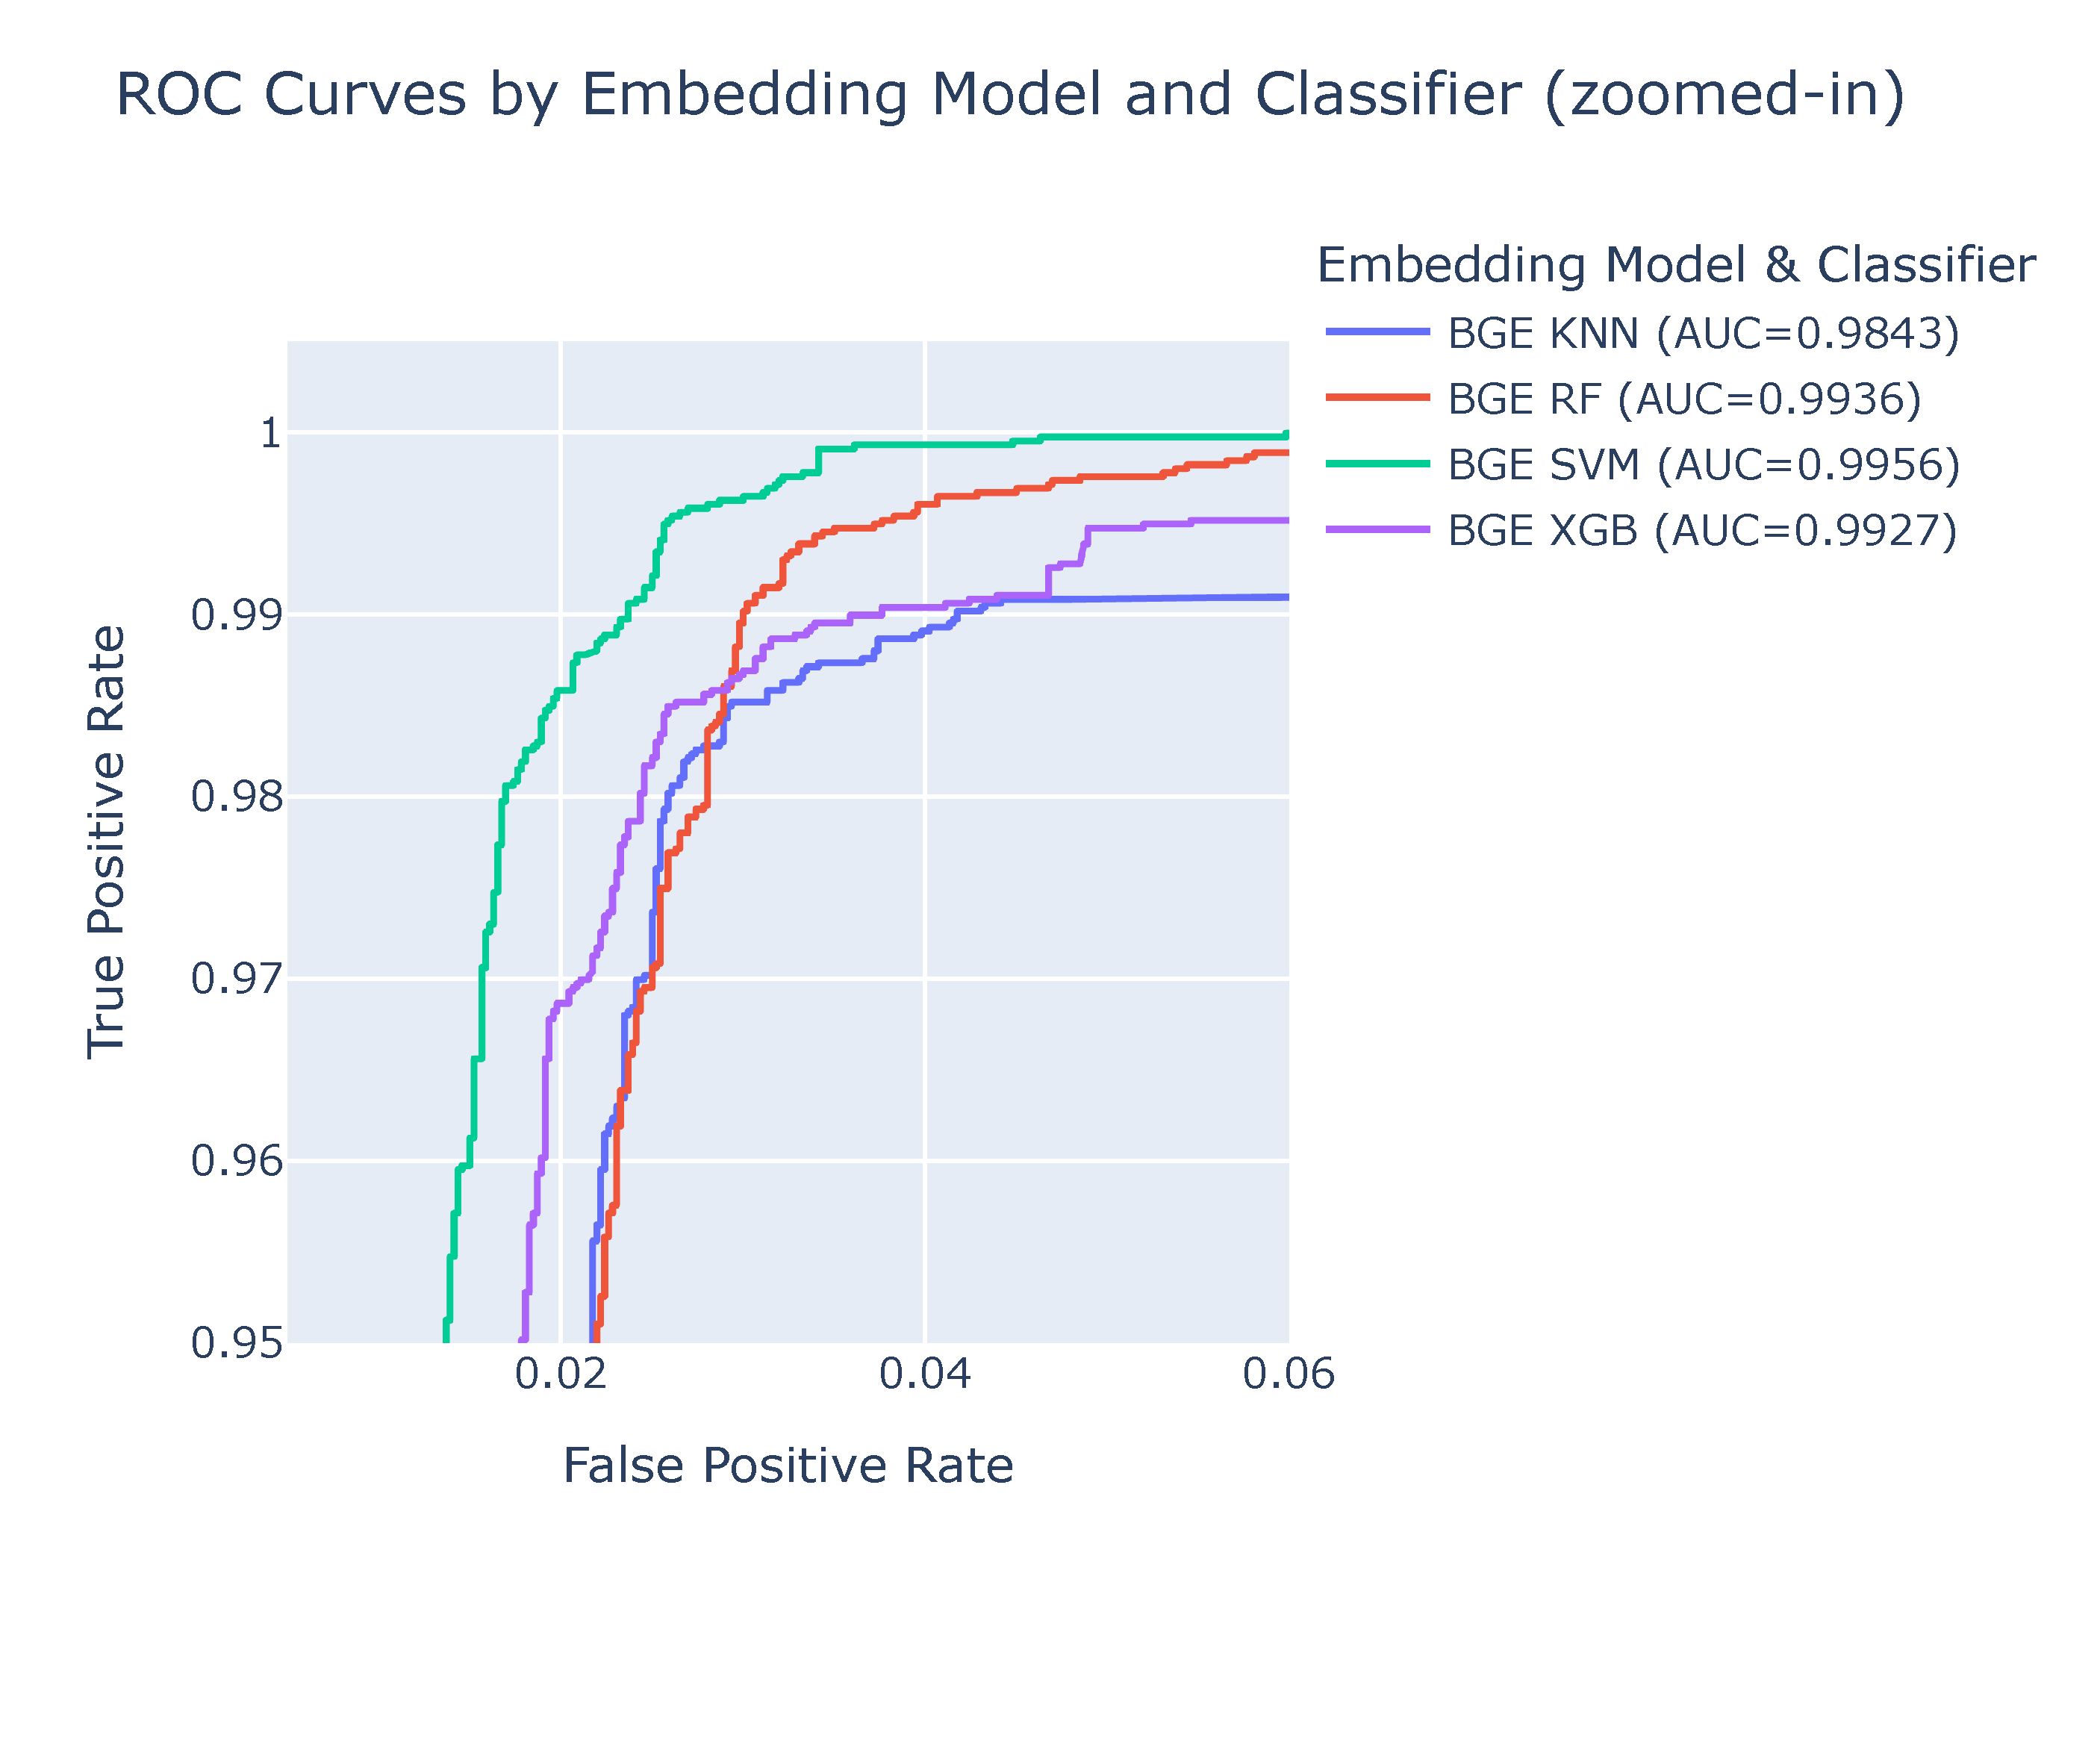
\includegraphics[width=0.37\textwidth,trim={18mm 50mm 180mm 50mm},clip]{roc_curves_bge_zoomed.pdf}\label{fig:bge_roc_zoomed}
    }
    \captionsetup[subfigure]{oneside,margin={-2.5cm,0cm}}
    \subfloat[Full Size]{
        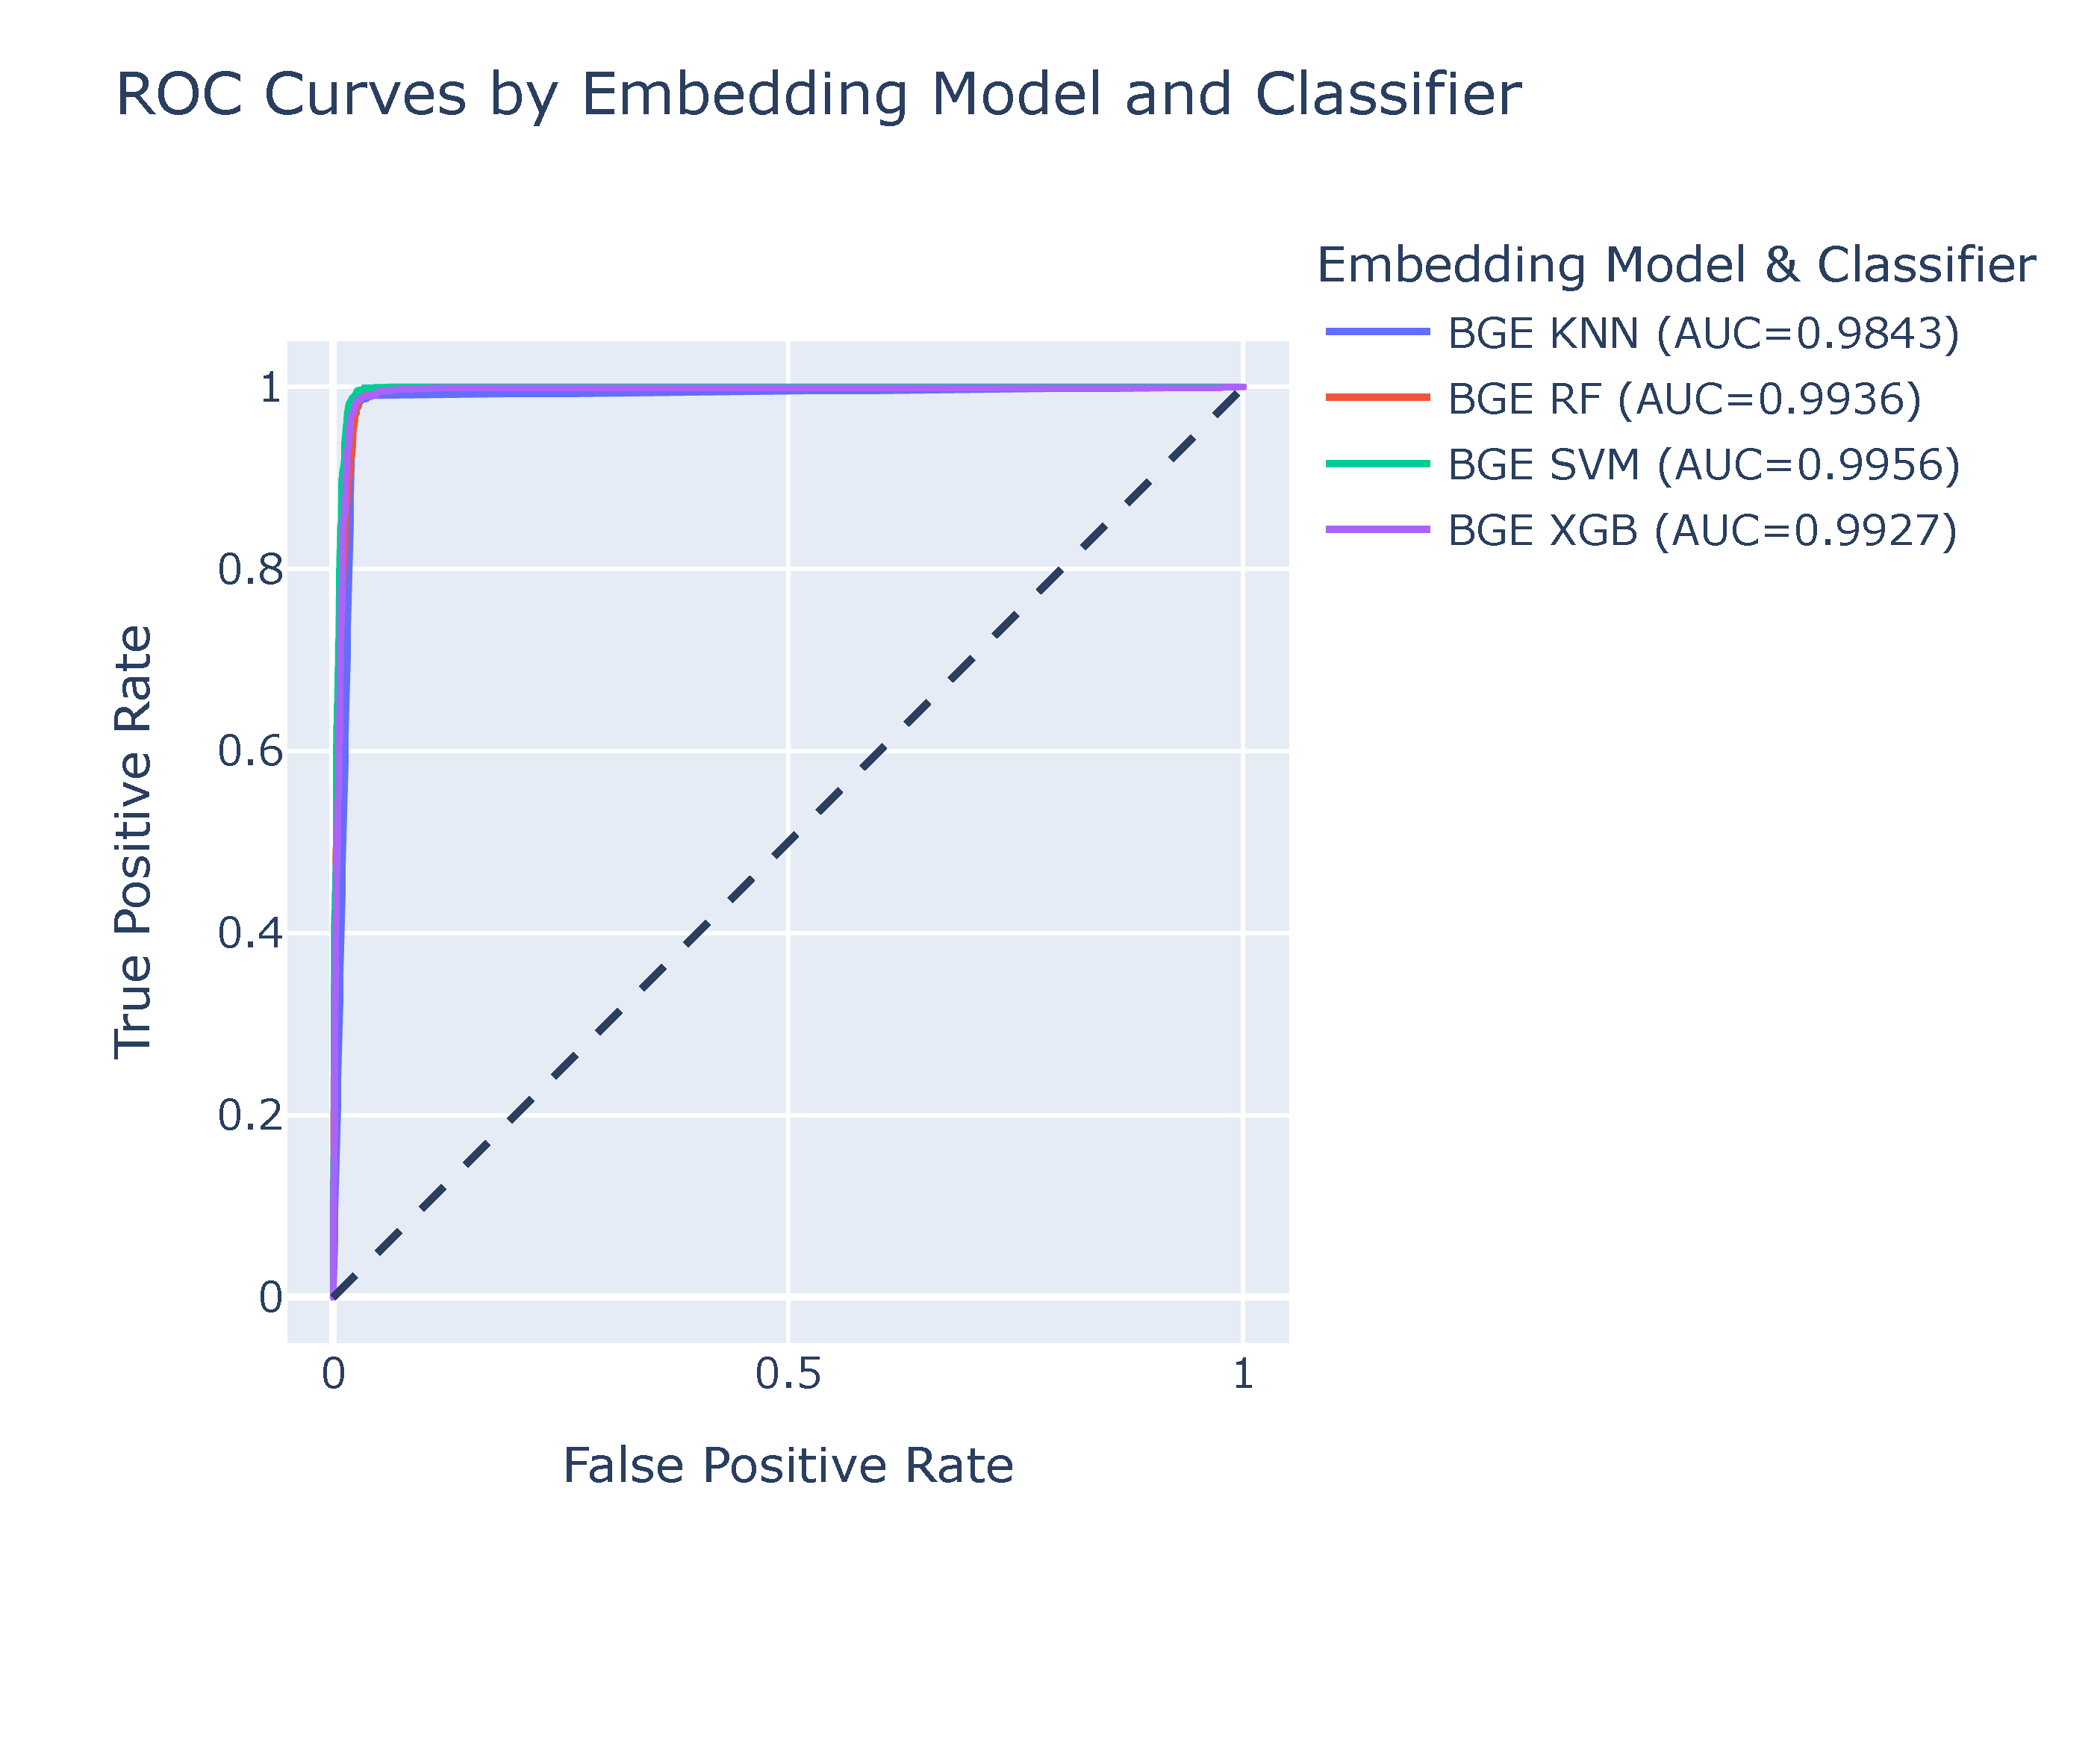
\includegraphics[width=0.58\textwidth,trim={25mm 50mm 12mm 50mm},clip]{roc_curves_bge.pdf}\label{fig:bge_roc_unzoomed}
    }
    \caption{BGE ROC Curves for Finalist Classifiers with Test Data}
\end{figure}

\begin{figure}[!h]
    \captionsetup{skip=5pt}
    \centering
    \captionsetup[subfigure]{oneside,margin={1cm,0cm}}
    \subfloat[Zoomed]{
        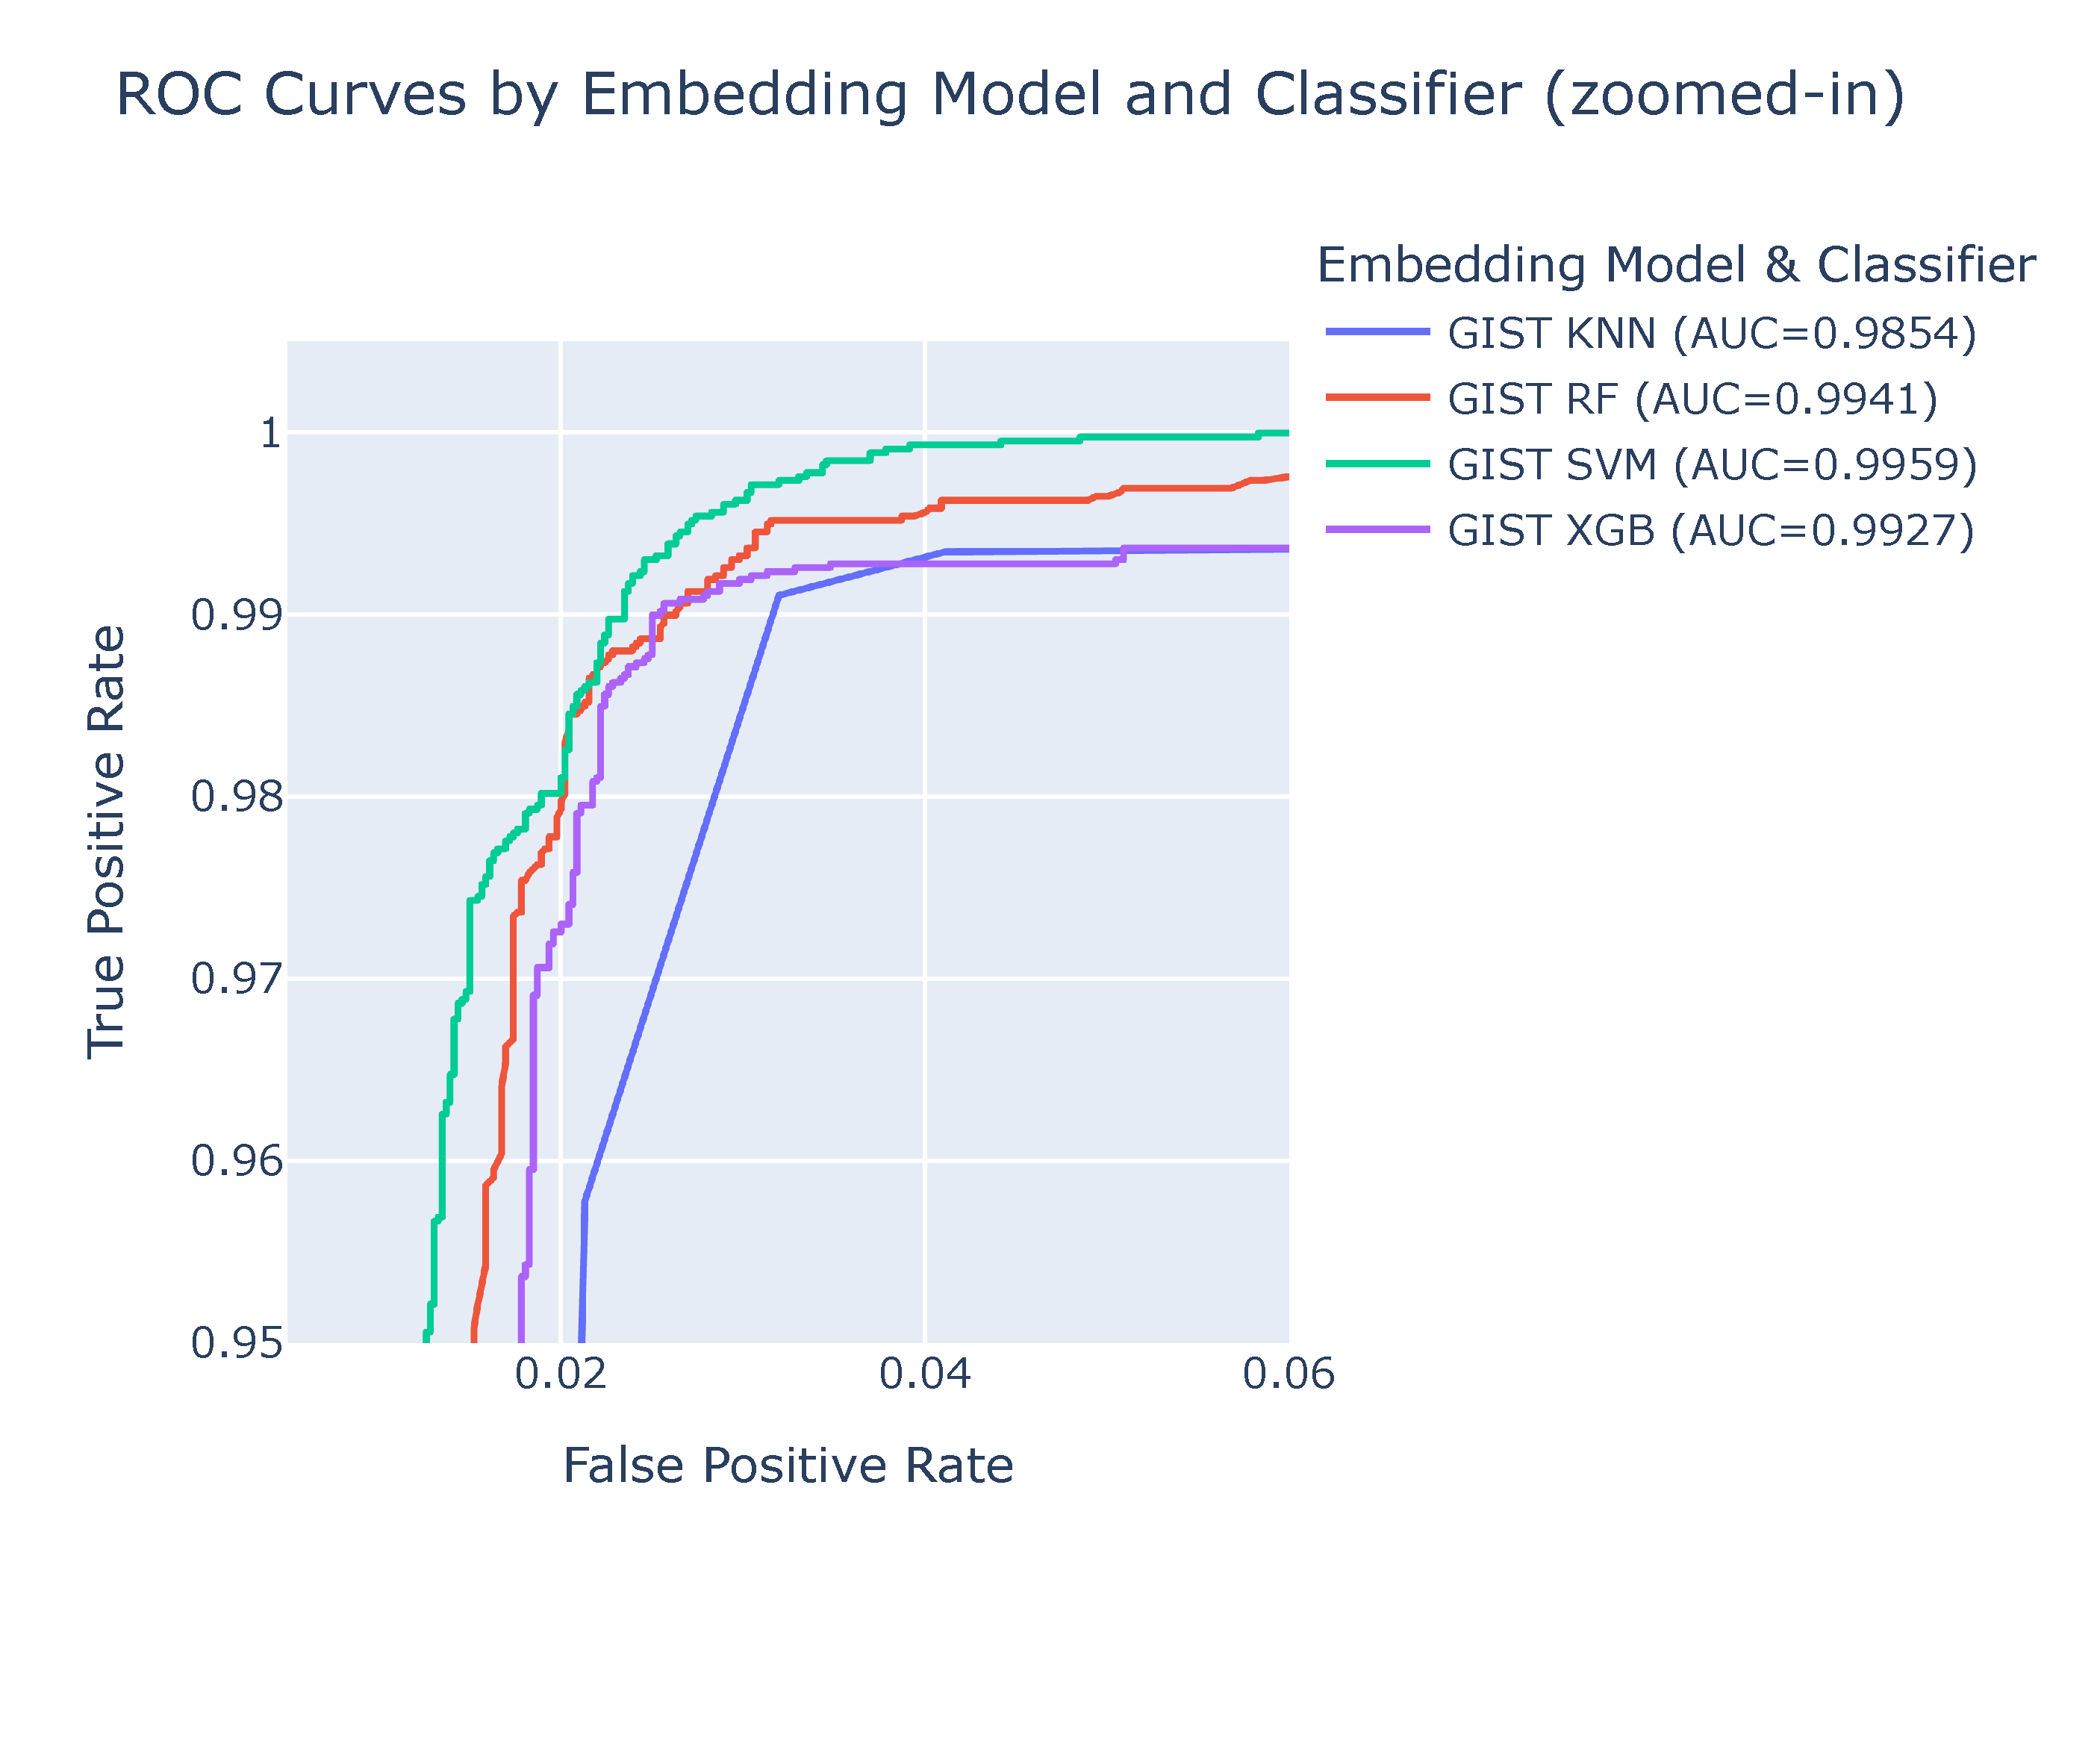
\includegraphics[width=0.37\textwidth,trim={18mm 50mm 180mm 50mm},clip]{roc_curves_gist_zoomed.pdf}\label{fig:gist_roc_zoomed}
    }
    \captionsetup[subfigure]{oneside,margin={-2.5cm,0cm}}
    \subfloat[Full Size]{
        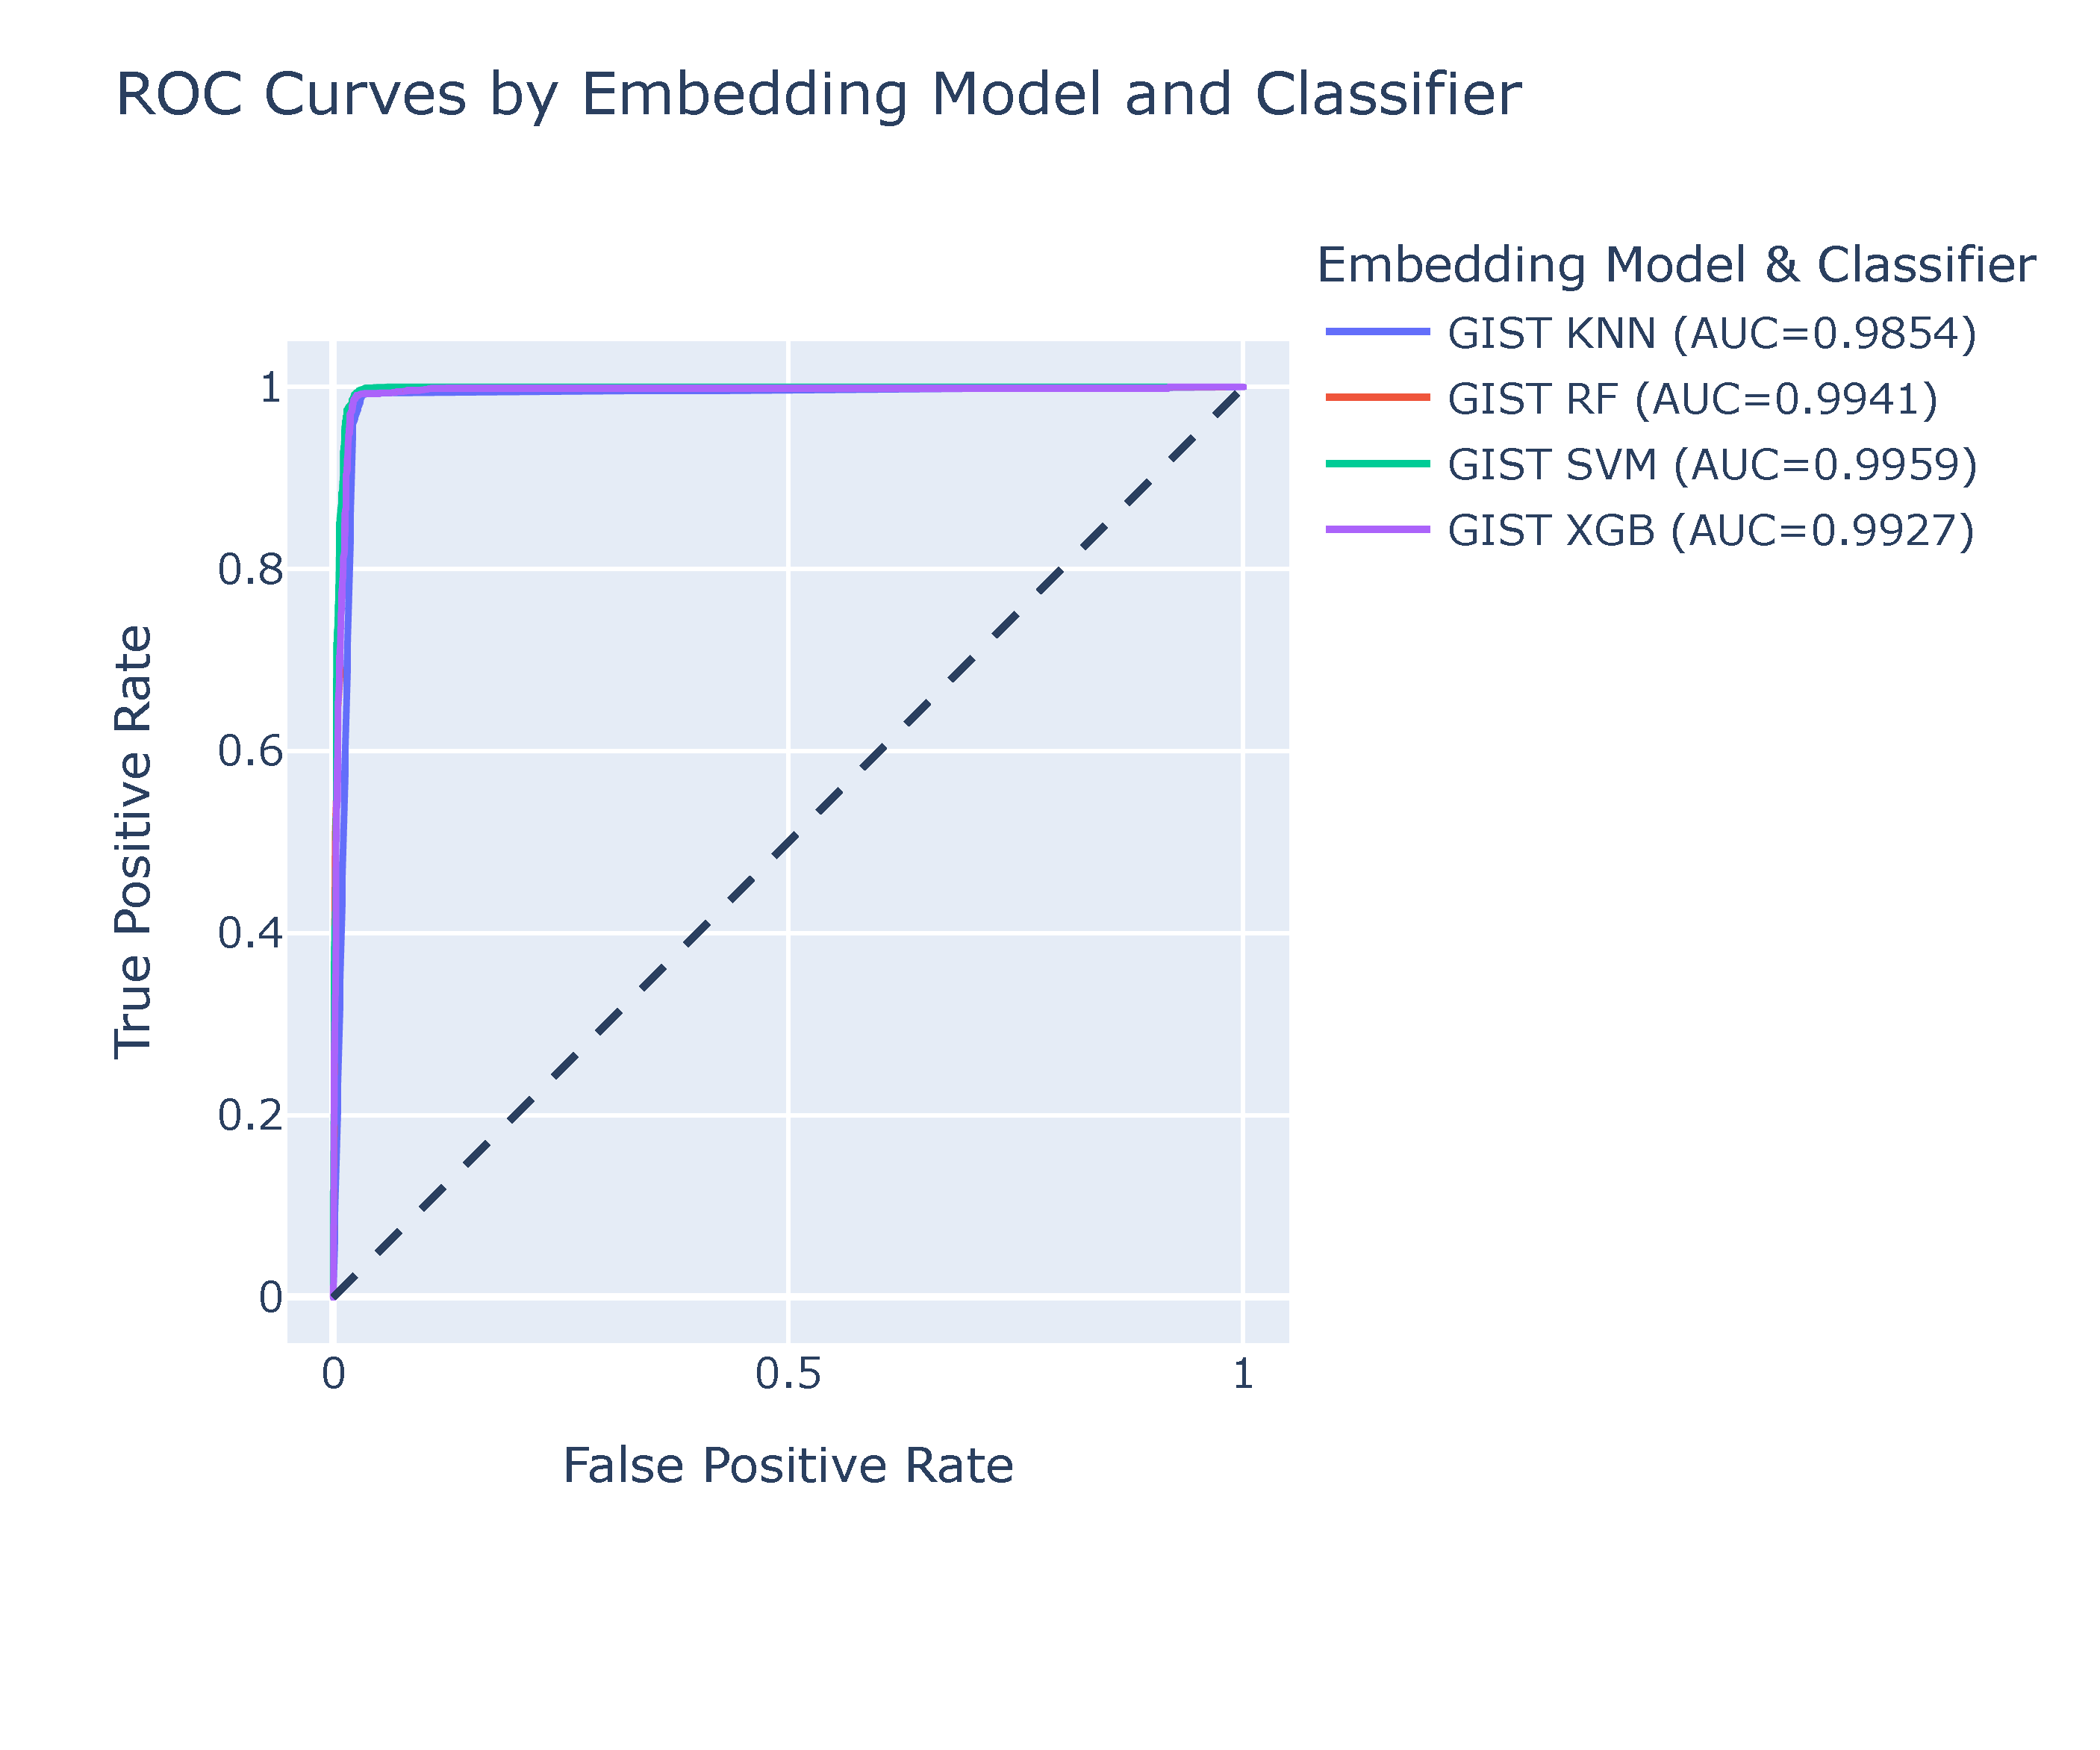
\includegraphics[width=0.58\textwidth,trim={25mm 50mm 12mm 50mm},clip]{roc_curves_gist.pdf}\label{fig:gist_roc_unzoomed}
    }
    \caption{GIST ROC Curves for Finalist Classifiers with Test Data}
\end{figure}

\begin{figure}[!h]
    \captionsetup{skip=5pt}
    \centering
    \captionsetup[subfigure]{oneside,margin={1cm,0cm}}
    \subfloat[Zoomed]{
        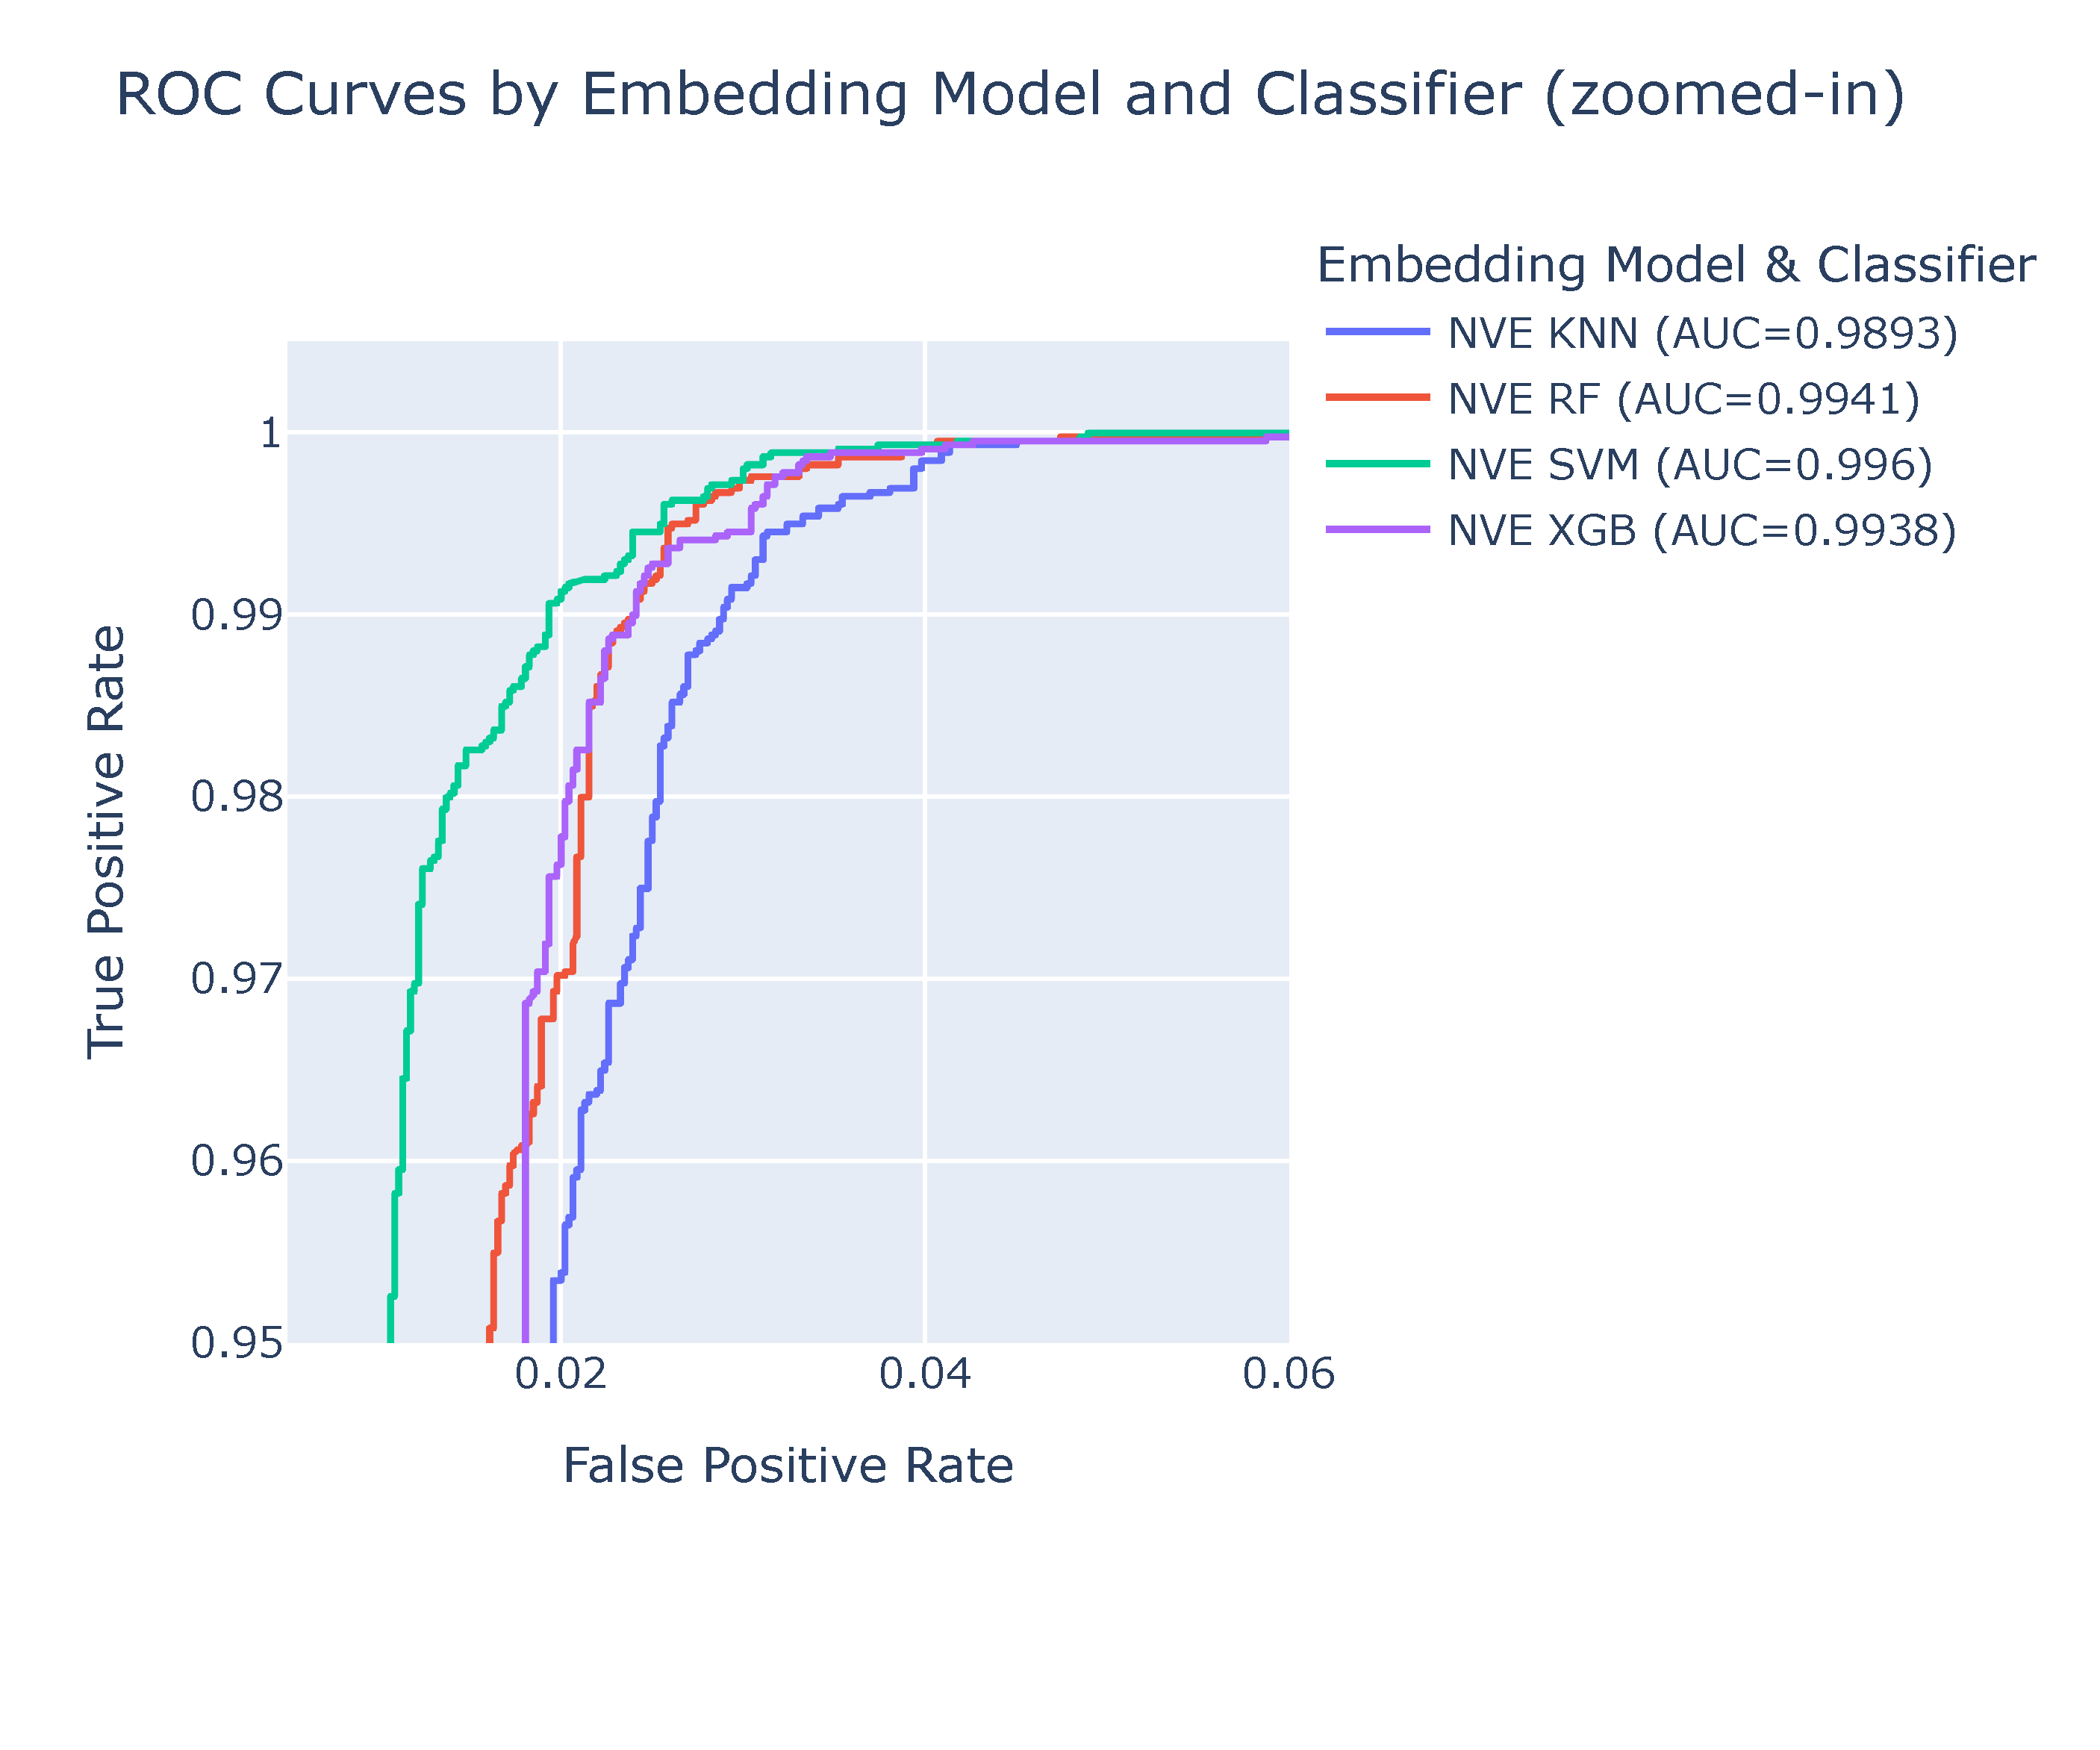
\includegraphics[width=0.37\textwidth,trim={18mm 50mm 180mm 50mm},clip]{roc_curves_nve_zoomed.pdf}\label{fig:nve_roc_zoomed}
    }
    \captionsetup[subfigure]{oneside,margin={-2.5cm,0cm}}
    \subfloat[Full Size]{
        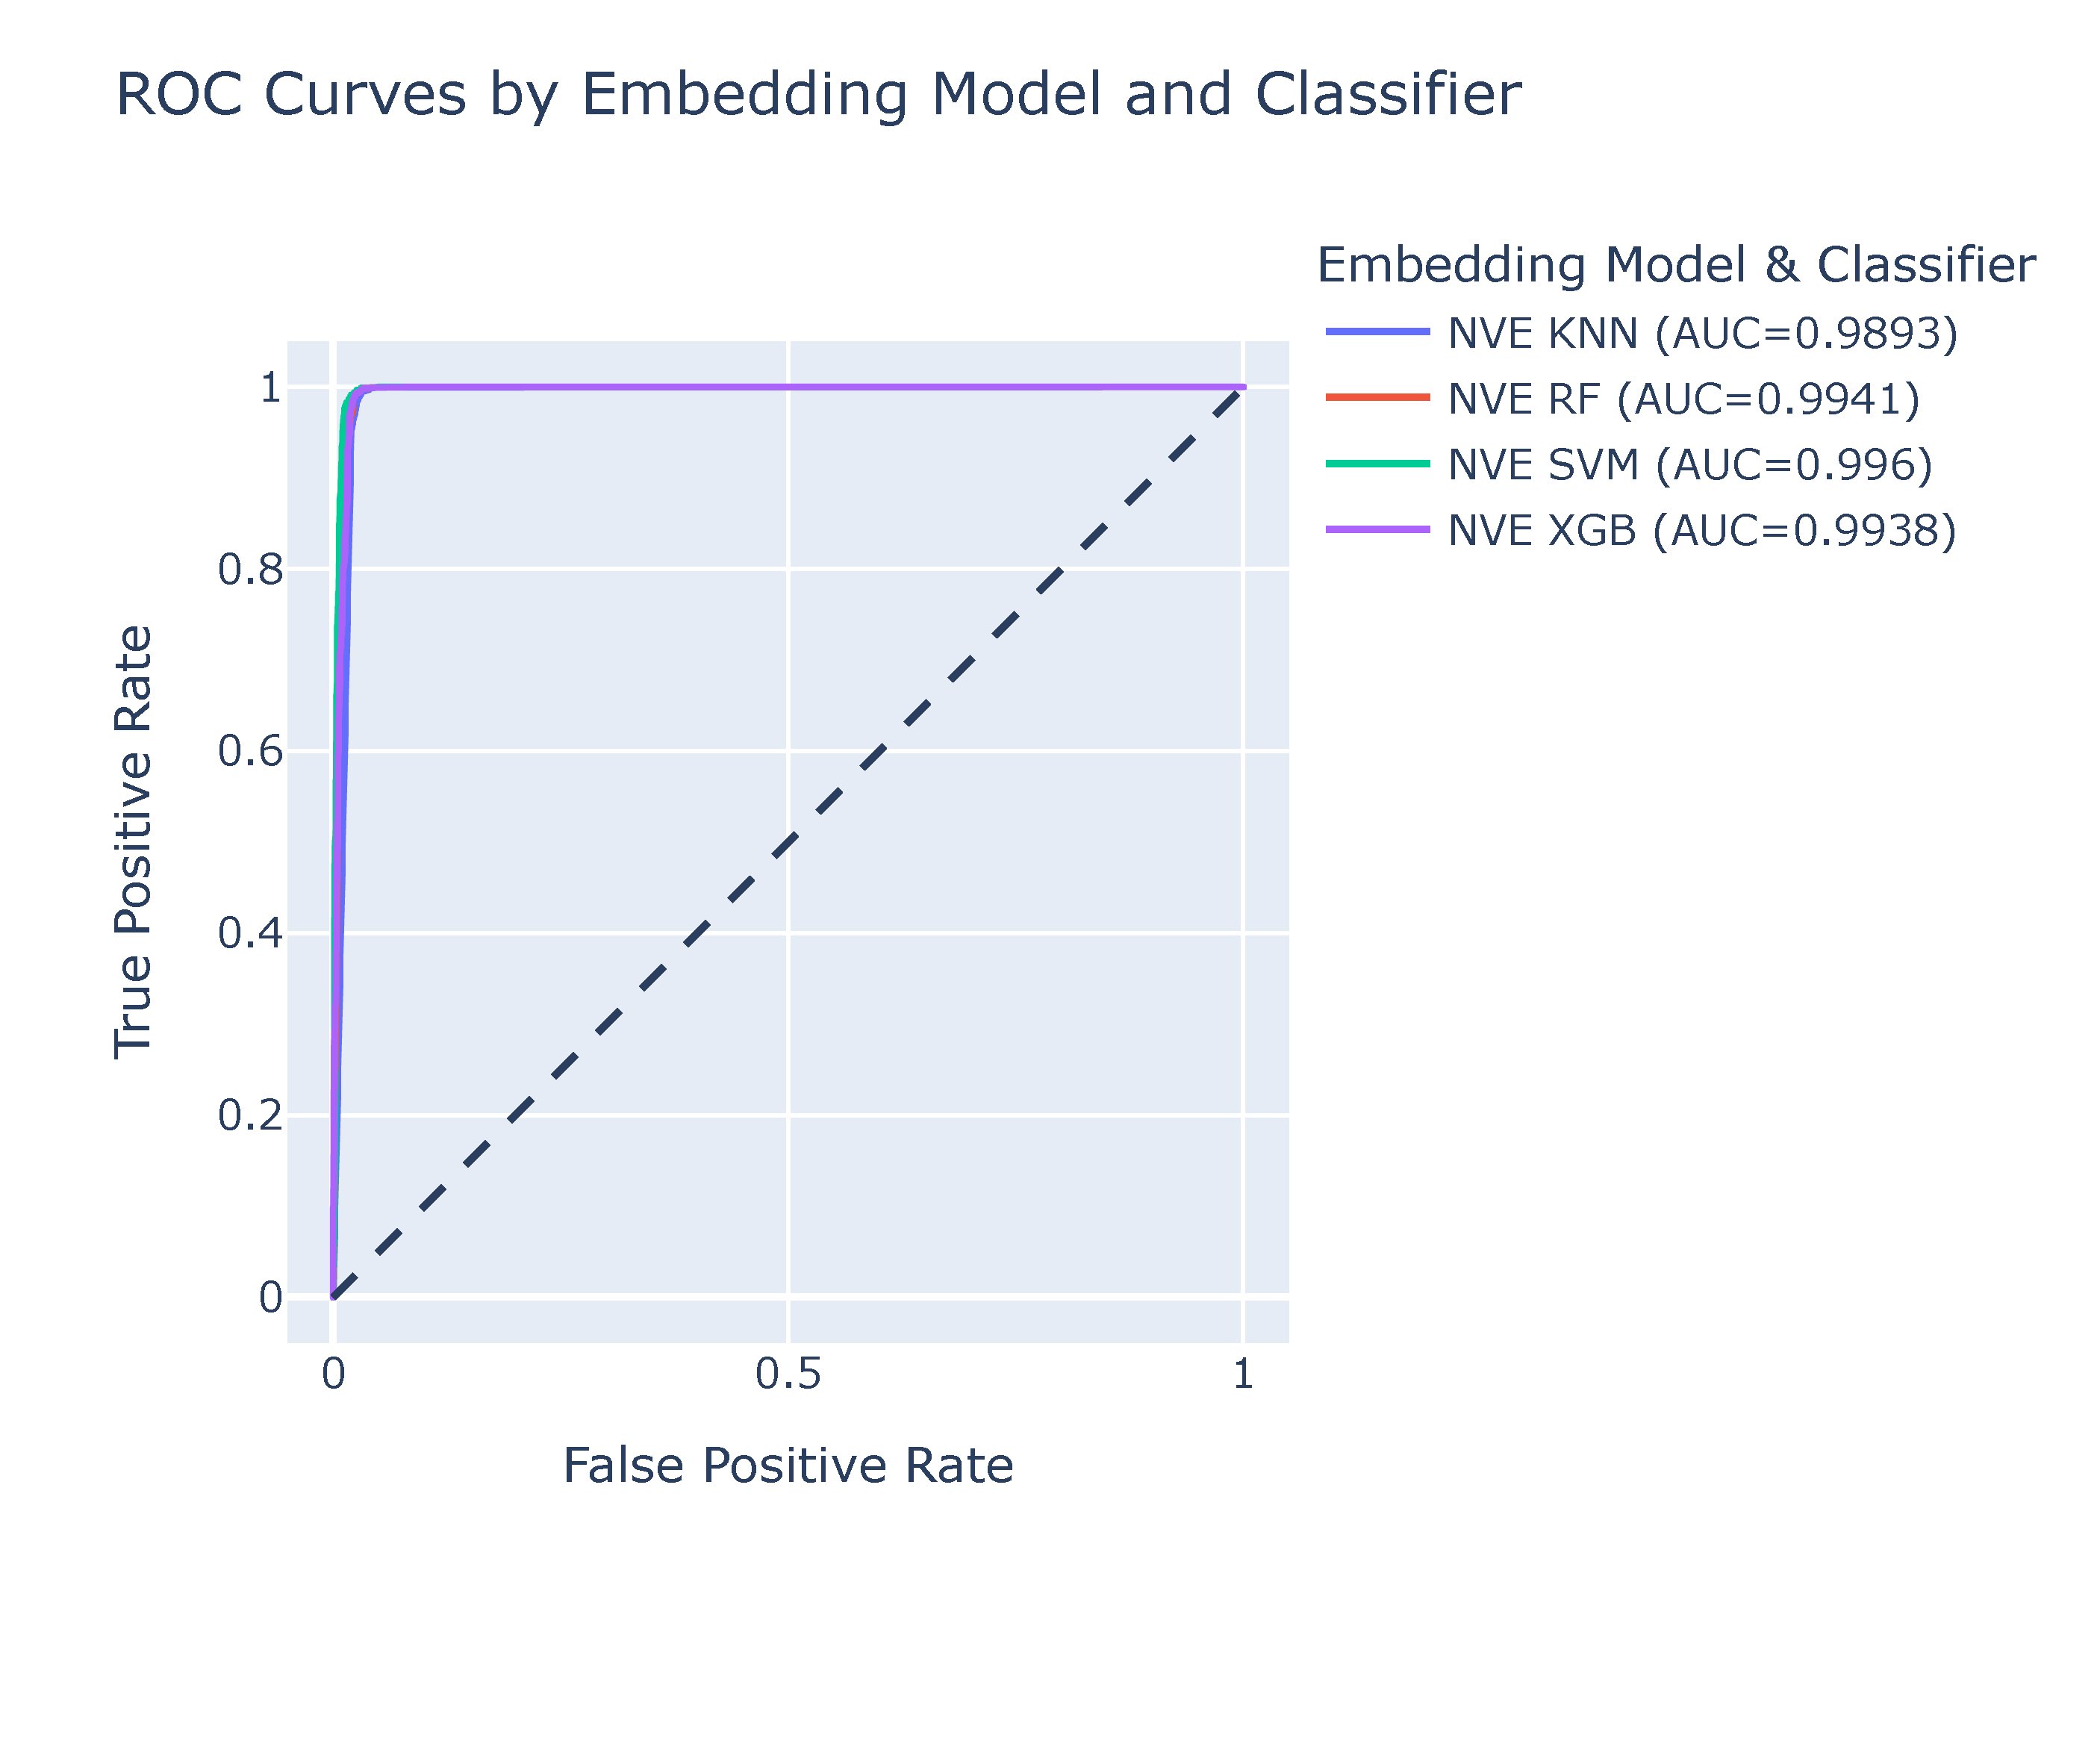
\includegraphics[width=0.58\textwidth,trim={25mm 50mm 12mm 50mm},clip]{roc_curves_nve.pdf}\label{fig:nve_roc_unzoomed}
    }
    \caption{NVE ROC Curves for Finalist Classifiers with Test Data}
\end{figure}

\begin{figure}[h!]
    \captionsetup{skip=5pt}
    \centering
    \captionsetup[subfigure]{oneside,margin={1cm,0cm}}
    \subfloat[Zoomed]{
        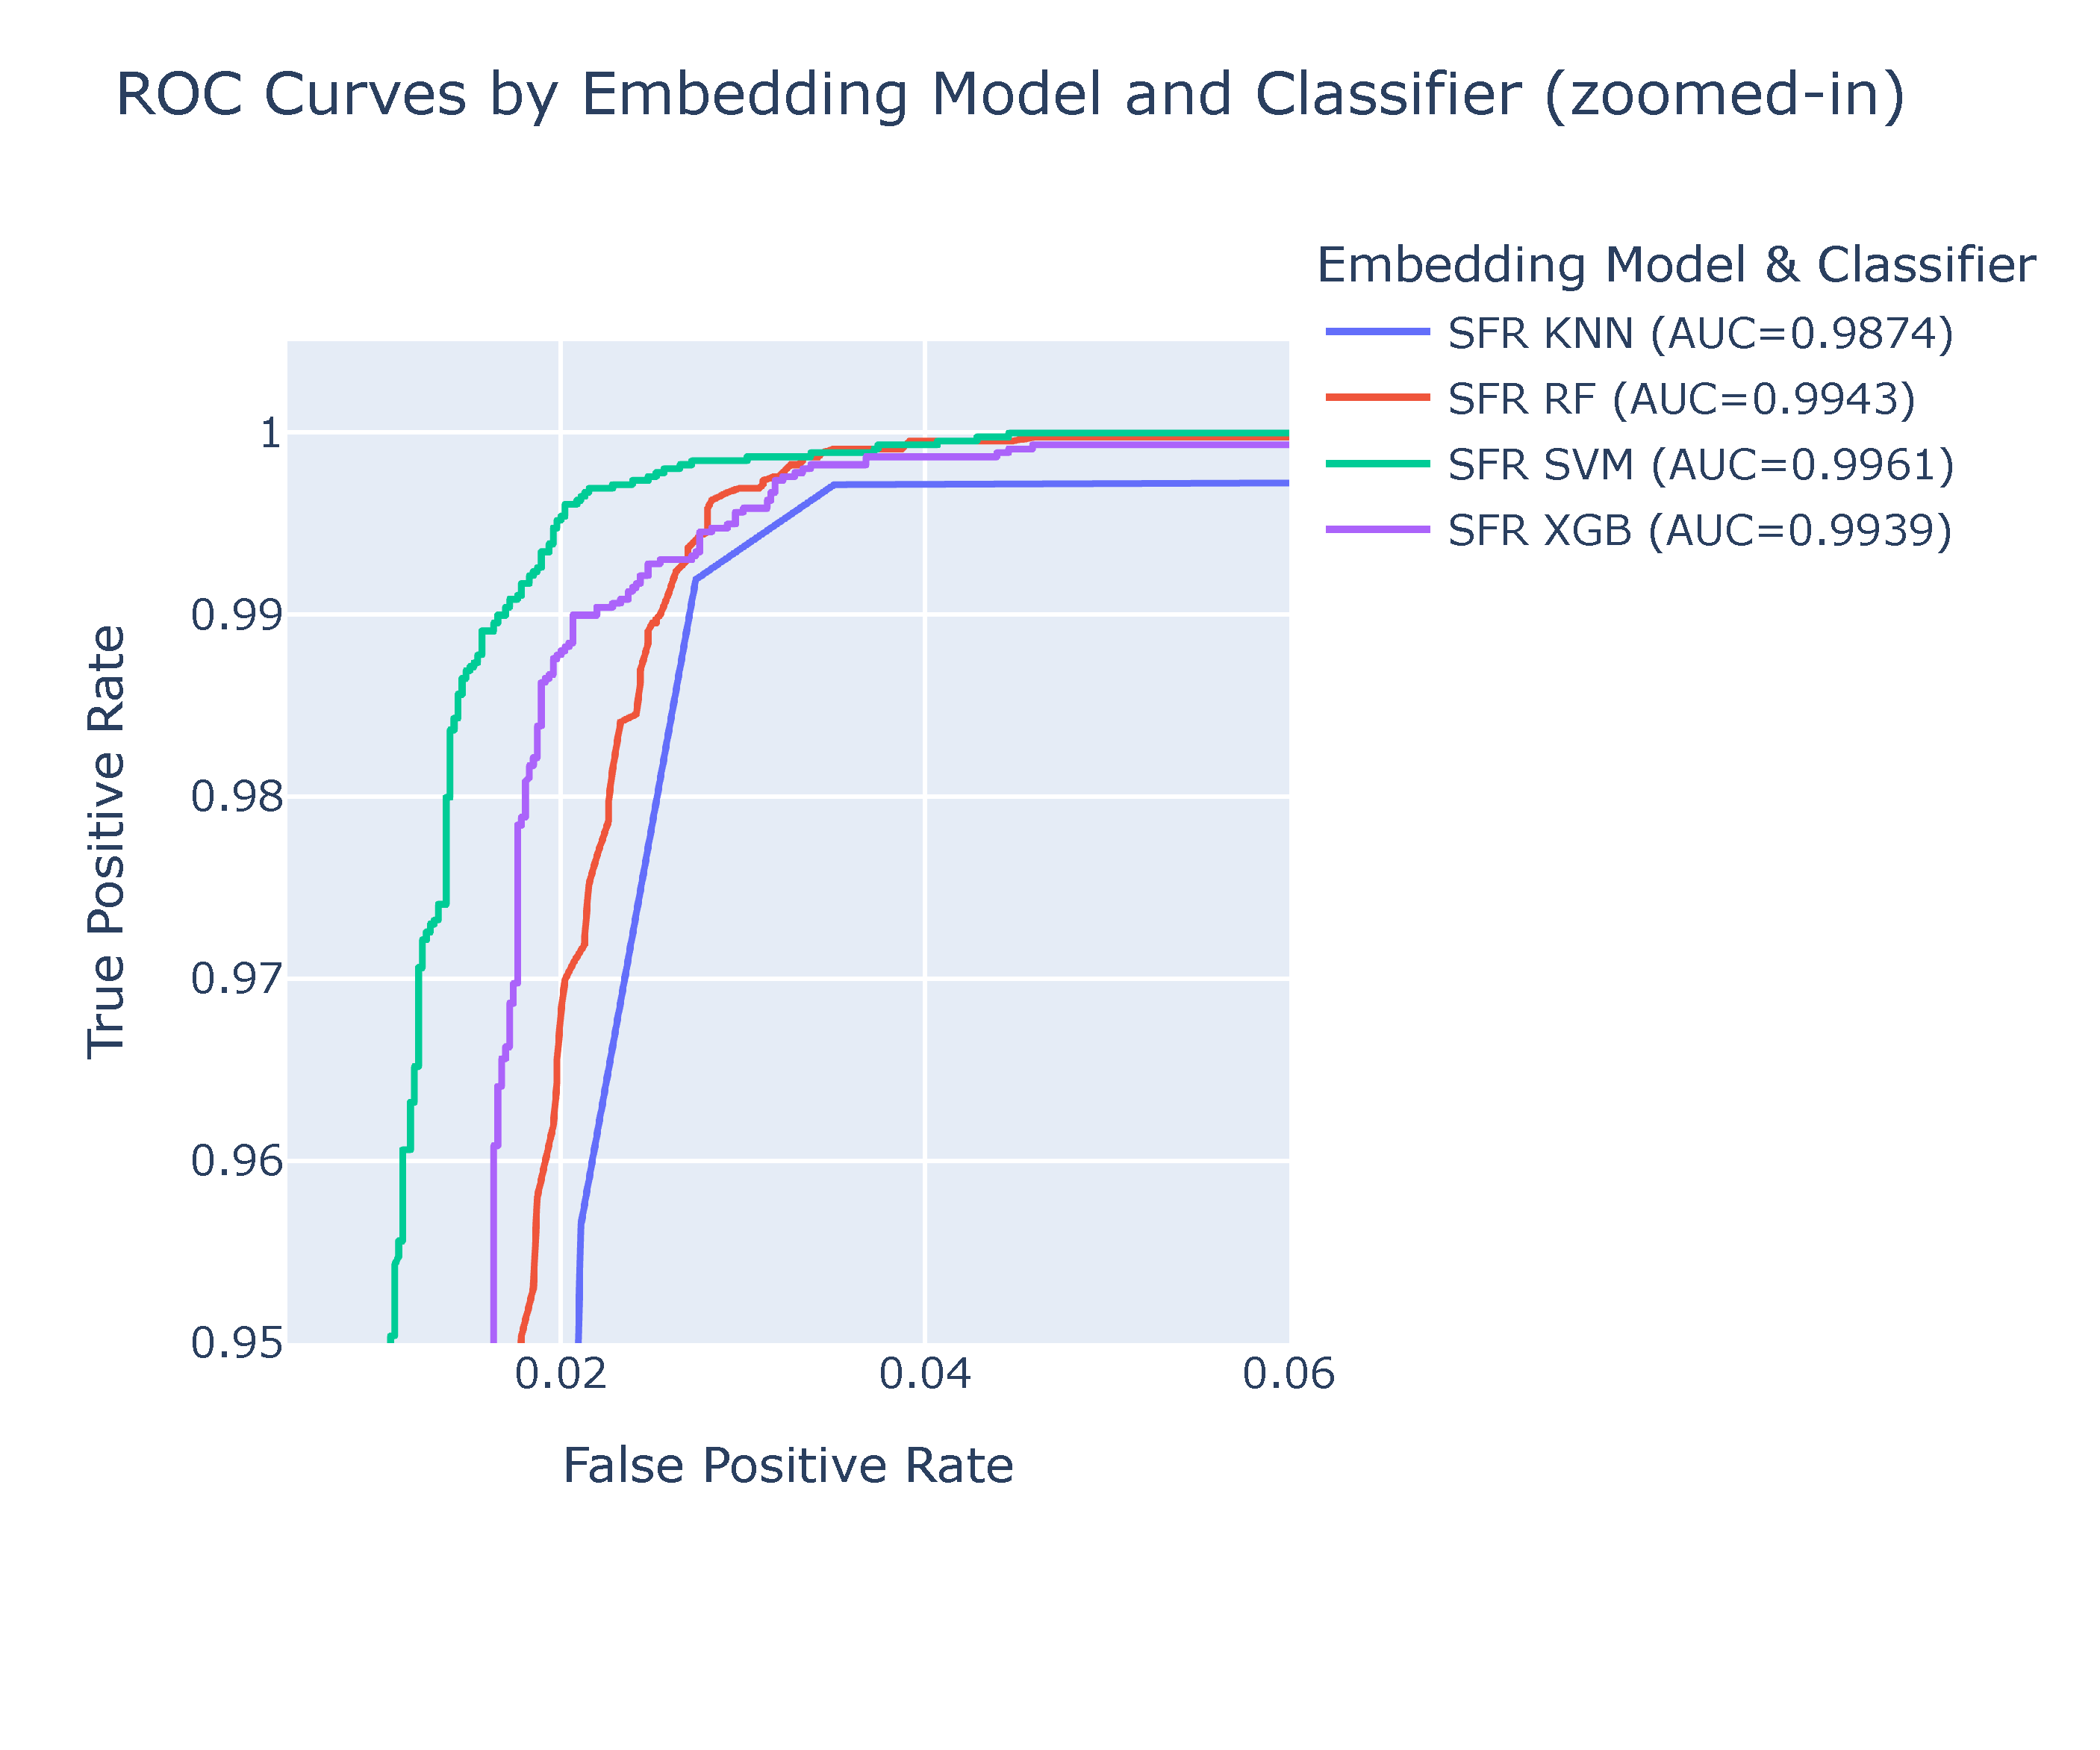
\includegraphics[width=0.37\textwidth,trim={18mm 50mm 180mm 50mm},clip]{roc_curves_sfr_zoomed.pdf}\label{fig:sfr_roc_zoomed}
    }
    \captionsetup[subfigure]{oneside,margin={-2.5cm,0cm}}
    \subfloat[Full Size]{
        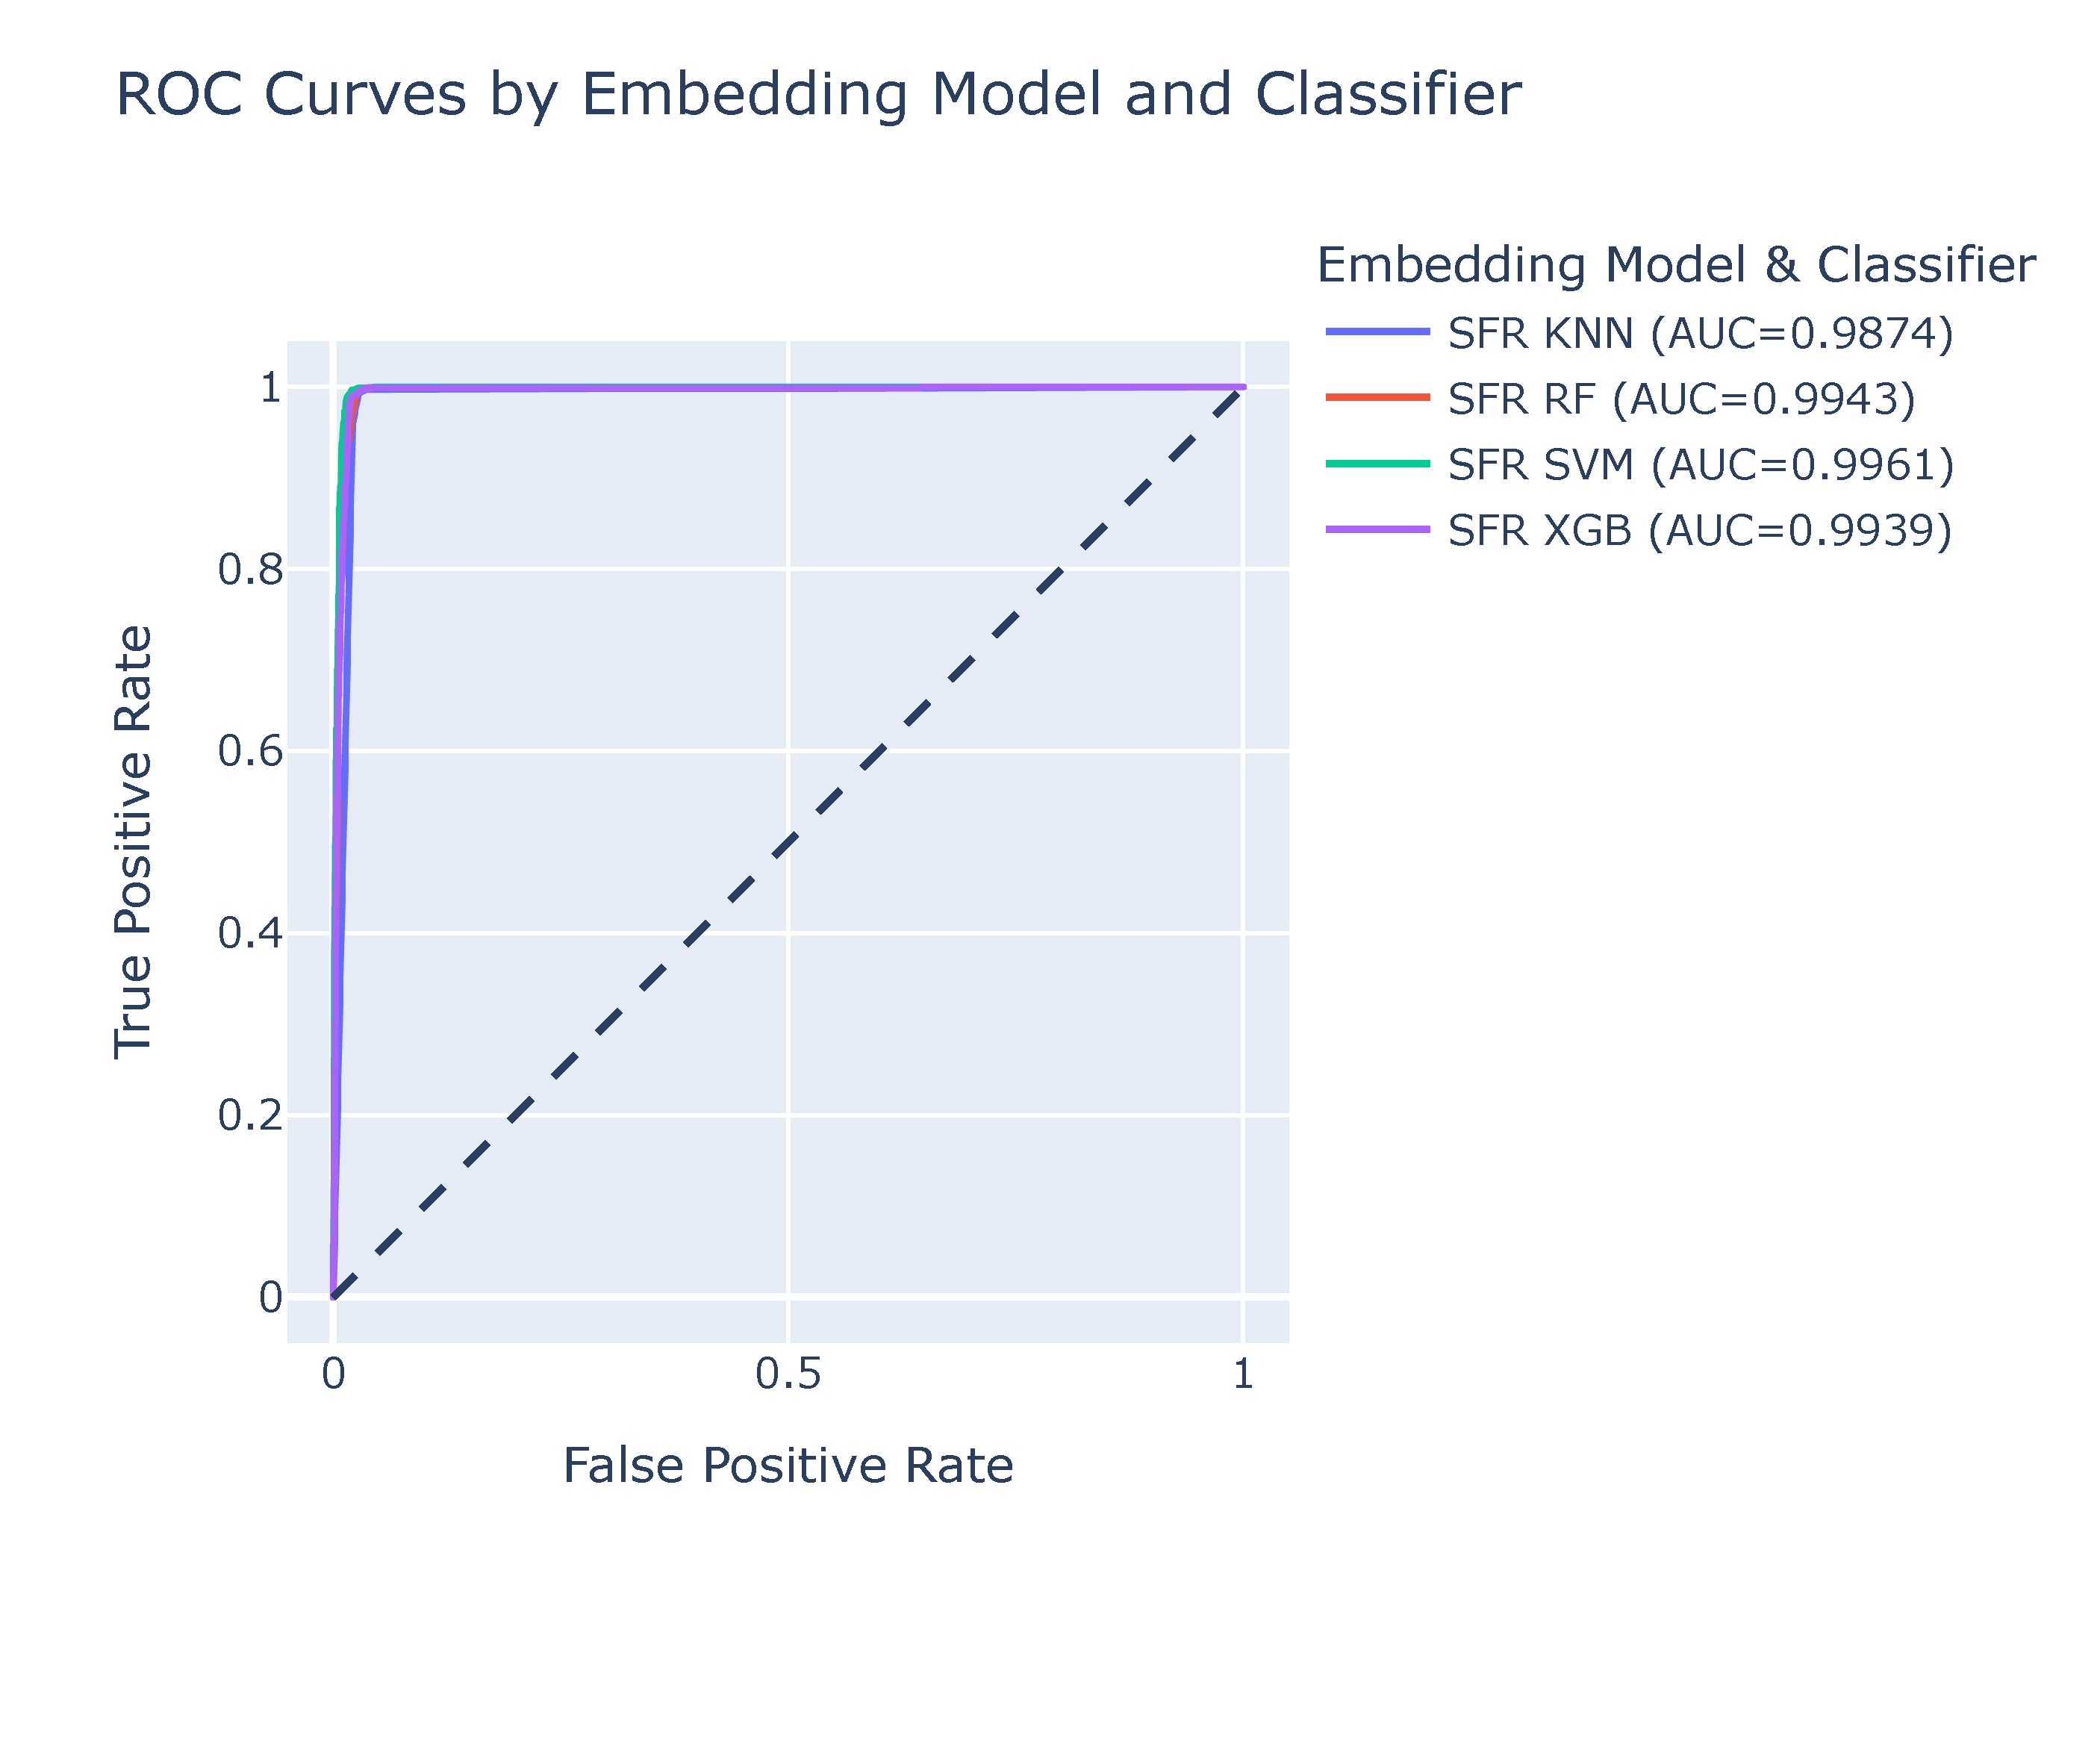
\includegraphics[width=0.58\textwidth,trim={25mm 50mm 12mm 50mm},clip]{roc_curves_sfr.pdf}\label{fig:sfr_roc_unzoomed}
    }
    \caption{SFR ROC Curves for Finalist Classifiers with Test Data}
\end{figure}

\clearpage
\section{Confusion Matrices}

\begin{figure}[!h]
    \captionsetup{skip=5pt}
    \centering
    \captionsetup[subfigure]{oneside,margin={1.3cm,0cm}}
    \subfloat[KNN]{
        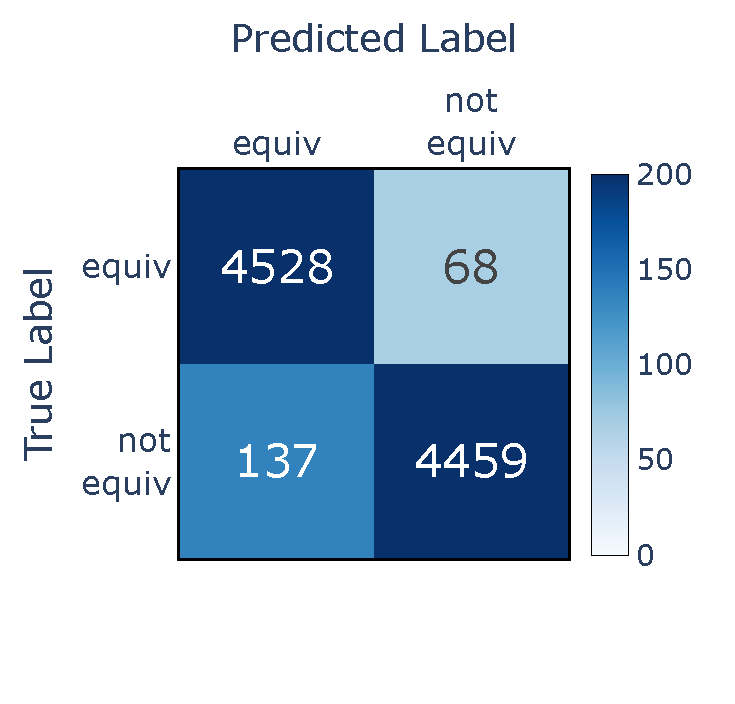
\includegraphics[width=0.277\textwidth,trim={0 23mm 26mm 0},clip]{cm_BGE_knn.pdf}
    }
    \captionsetup[subfigure]{oneside,margin={0cm,0cm}}
    \subfloat[Random Forest]{
        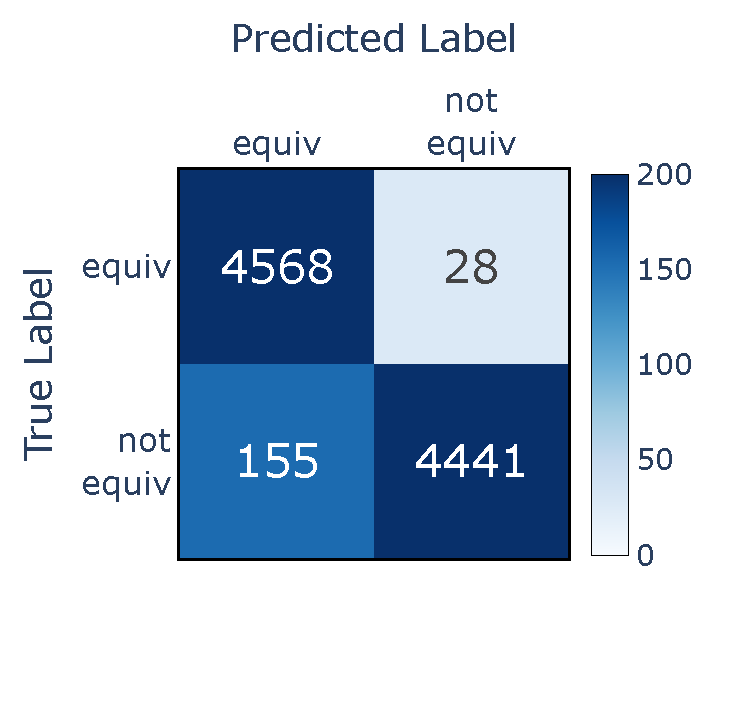
\includegraphics[width=0.194\textwidth,trim={29mm 23mm 26mm 0},clip]{cm_BGE_rf.pdf}
    }
    \captionsetup[subfigure]{oneside,margin={0cm,0cm}}
    \subfloat[SVM]{
        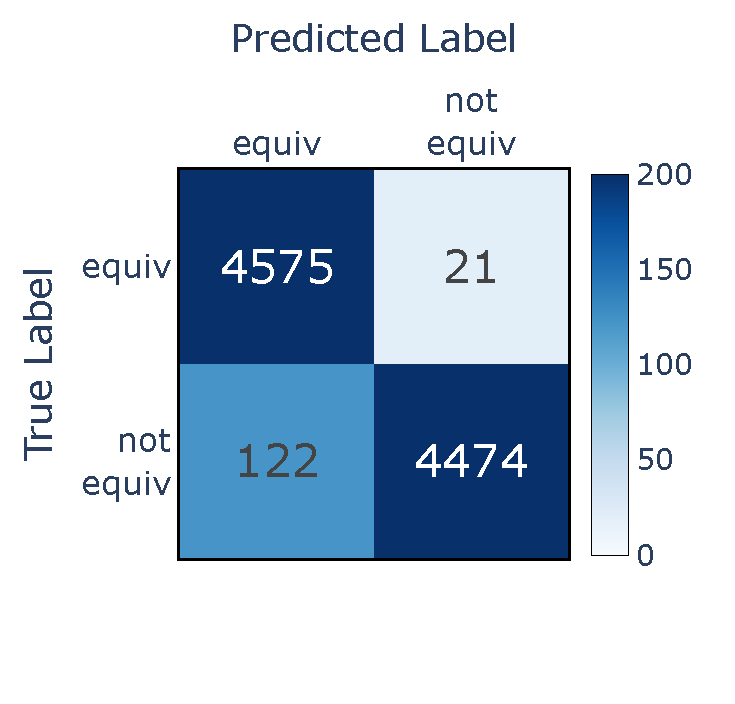
\includegraphics[width=0.194\textwidth,trim={29mm 23mm 26mm 0},clip]{cm_BGE_svm.pdf}
    }
    \captionsetup[subfigure]{oneside,margin={-1.25cm,0cm}}
    \subfloat[XGBoost]{
        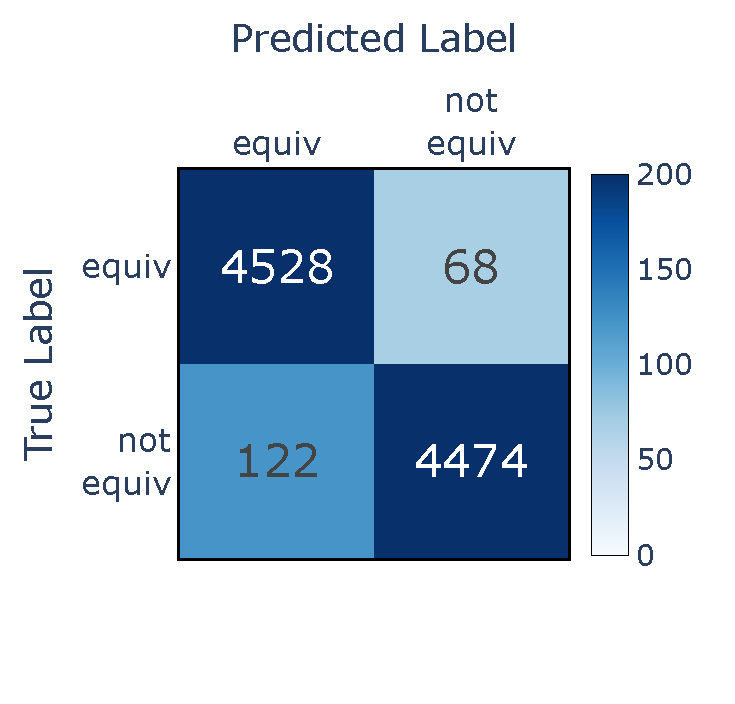
\includegraphics[width=0.246\textwidth,trim={29mm 23mm 7mm 0},clip]{cm_BGE_xgb.pdf}
    }
    \caption{BGE Confusion Matrices for Finalist Classifiers with Test Data}
\end{figure}

\begin{figure}[!h]
    \captionsetup{skip=5pt}
    \centering
    \captionsetup[subfigure]{oneside,margin={1.3cm,0cm}}
    \subfloat[KNN]{
        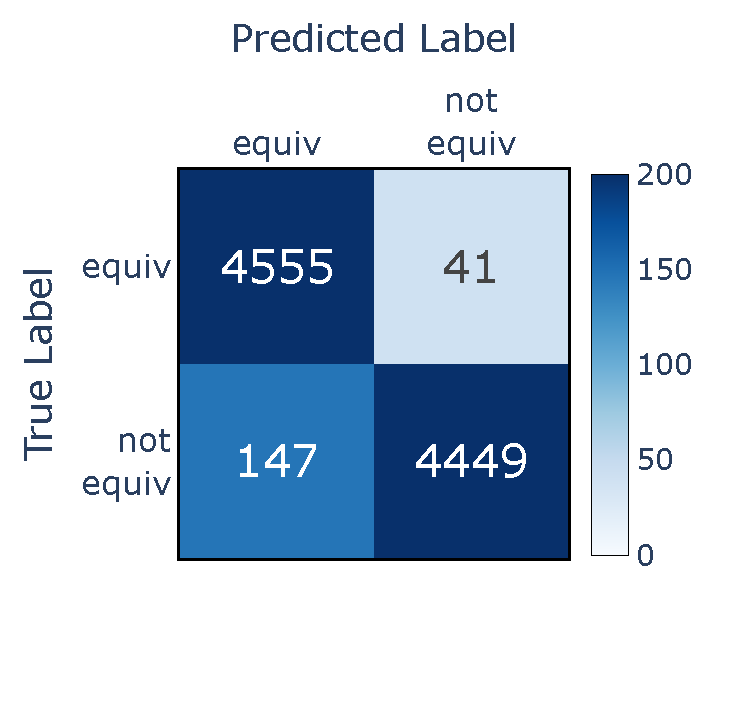
\includegraphics[width=0.277\textwidth,trim={0 23mm 26mm 0},clip]{cm_GIST_knn.pdf}
    }
    \captionsetup[subfigure]{oneside,margin={0cm,0cm}}
    \subfloat[Random Forest]{
        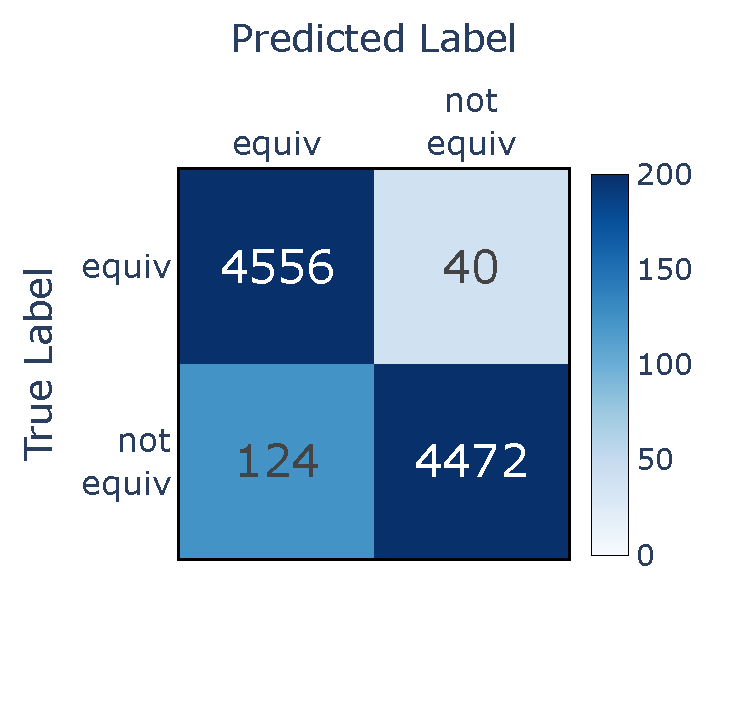
\includegraphics[width=0.194\textwidth,trim={29mm 23mm 26mm 0},clip]{cm_GIST_rf.pdf}
    }
    \captionsetup[subfigure]{oneside,margin={0cm,0cm}}
    \subfloat[SVM]{
        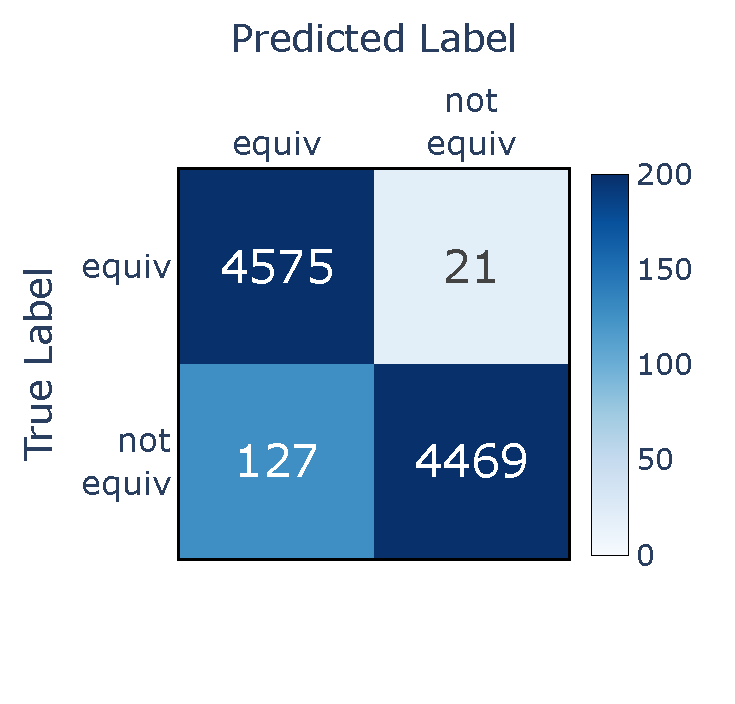
\includegraphics[width=0.194\textwidth,trim={29mm 23mm 26mm 0},clip]{cm_GIST_svm.pdf}
    }
    \captionsetup[subfigure]{oneside,margin={-1.25cm,0cm}}
    \subfloat[XGBoost]{
        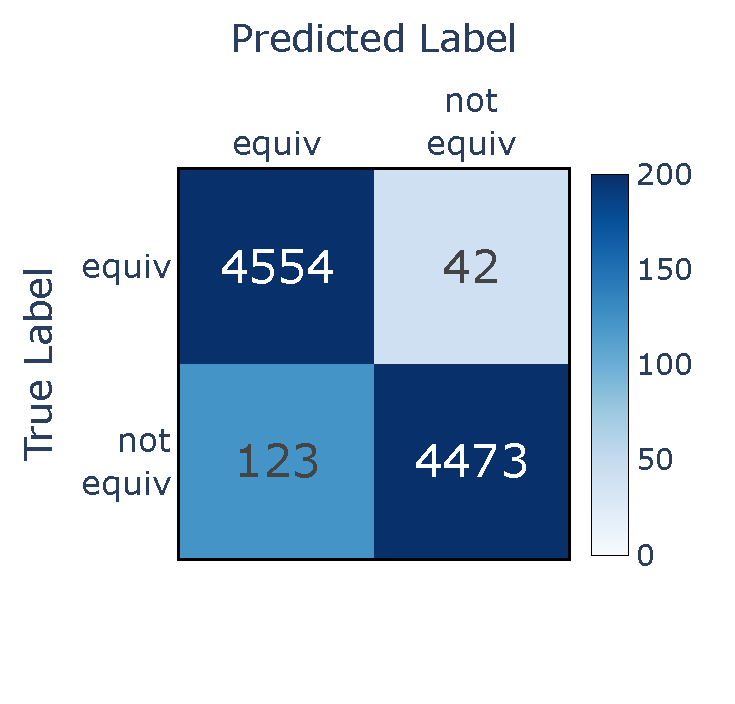
\includegraphics[width=0.246\textwidth,trim={29mm 23mm 7mm 0},clip]{cm_GIST_xgb.pdf}
    }
    \caption{GIST Confusion Matrices for Finalist Classifiers with Test Data}
\end{figure}

\begin{figure}[!h]
    \captionsetup{skip=5pt}
    \centering
    \captionsetup[subfigure]{oneside,margin={1.3cm,0cm}}
    \subfloat[KNN]{
        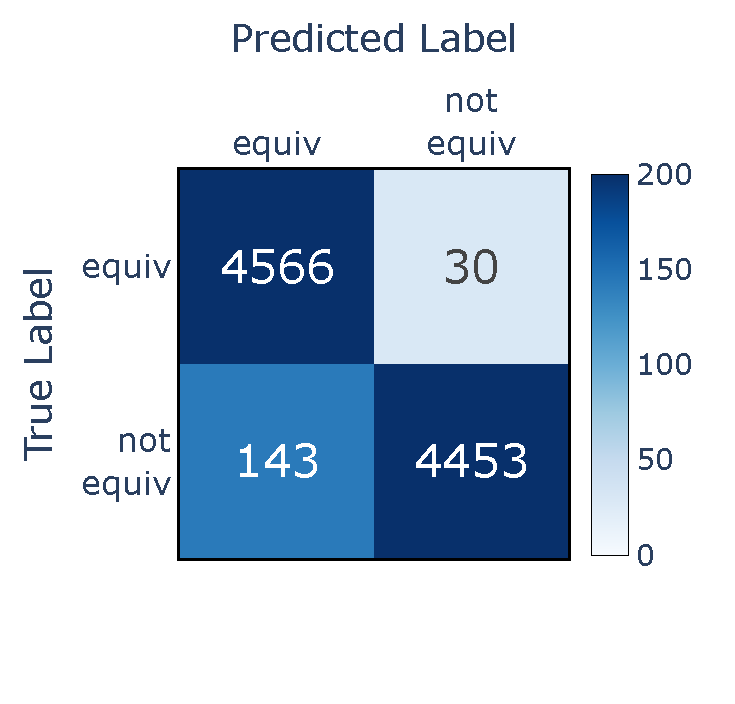
\includegraphics[width=0.277\textwidth,trim={0 23mm 26mm 0},clip]{cm_NVE_knn.pdf}
    }
    \captionsetup[subfigure]{oneside,margin={0cm,0cm}}
    \subfloat[Random Forest]{
        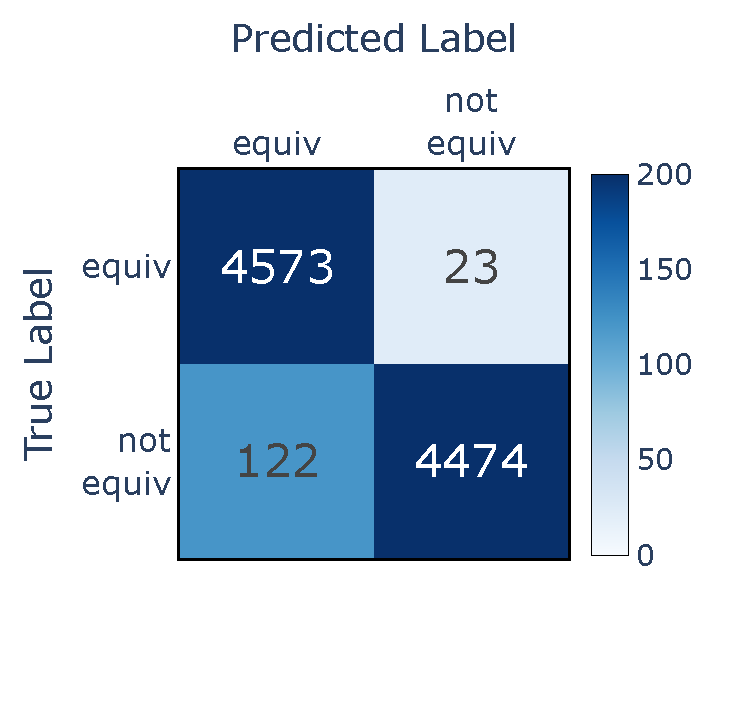
\includegraphics[width=0.194\textwidth,trim={29mm 23mm 26mm 0},clip]{cm_NVE_rf.pdf}
    }
    \captionsetup[subfigure]{oneside,margin={0cm,0cm}}
    \subfloat[SVM]{
        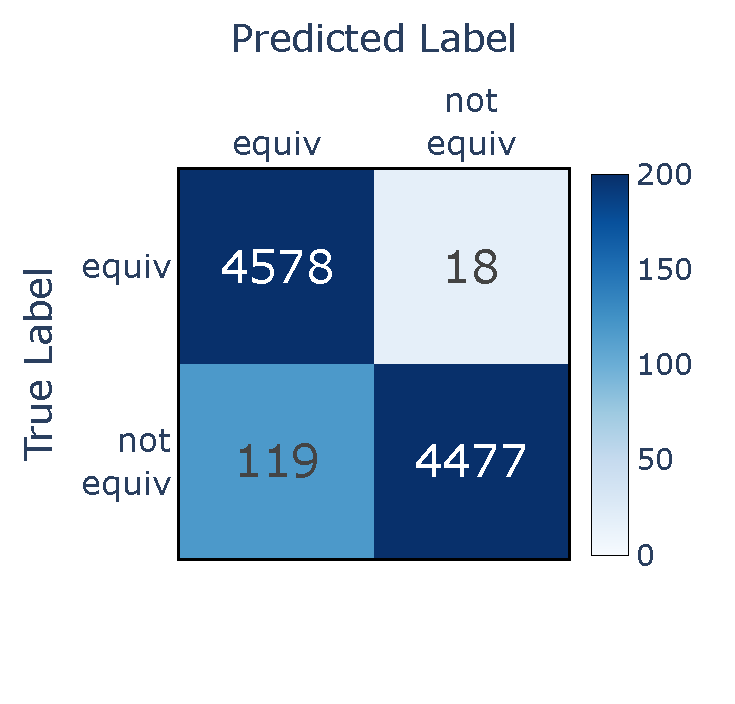
\includegraphics[width=0.194\textwidth,trim={29mm 23mm 26mm 0},clip]{cm_NVE_svm.pdf}
    }
    \captionsetup[subfigure]{oneside,margin={-1.25cm,0cm}}
    \subfloat[XGBoost]{
        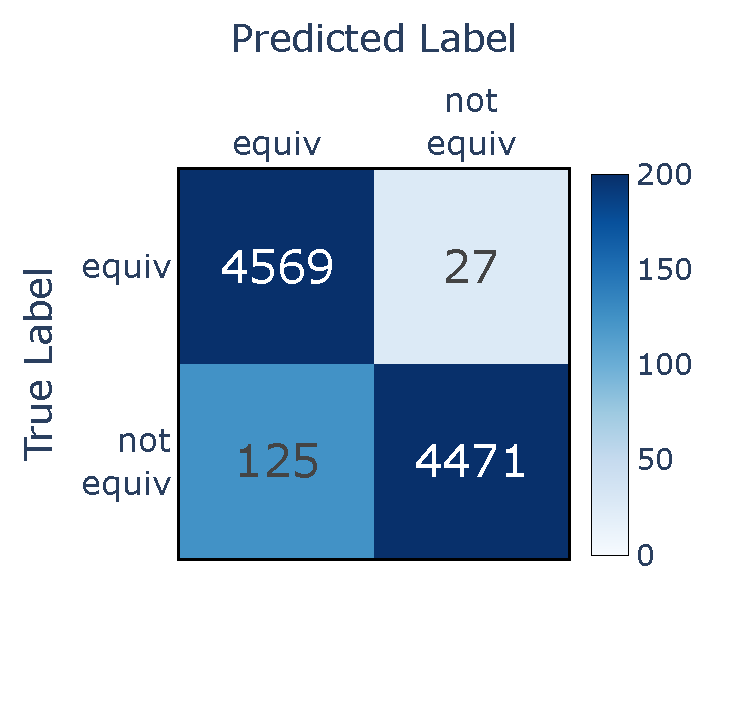
\includegraphics[width=0.246\textwidth,trim={29mm 23mm 7mm 0},clip]{cm_NVE_xgb.pdf}
    }
    \caption{NVE Confusion Matrices for Finalist Classifiers with Test Data}
\end{figure}

\begin{figure}[!h]
    \captionsetup{skip=5pt}
    \centering
    \captionsetup[subfigure]{oneside,margin={1.3cm,0cm}}
    \subfloat[KNN]{
        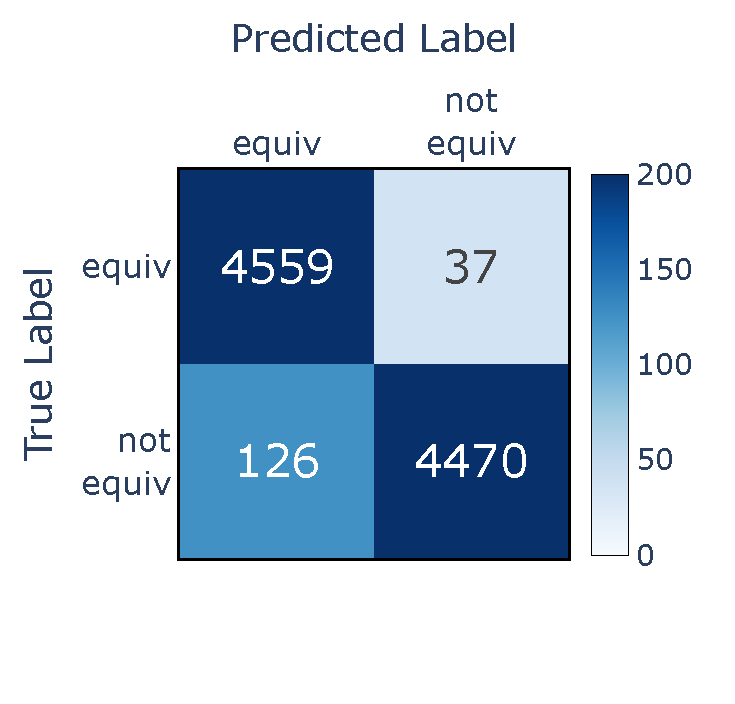
\includegraphics[width=0.277\textwidth,trim={0 23mm 26mm 0},clip]{cm_SFR_knn.pdf}
    }
    \captionsetup[subfigure]{oneside,margin={0cm,0cm}}
    \subfloat[Random Forest]{
        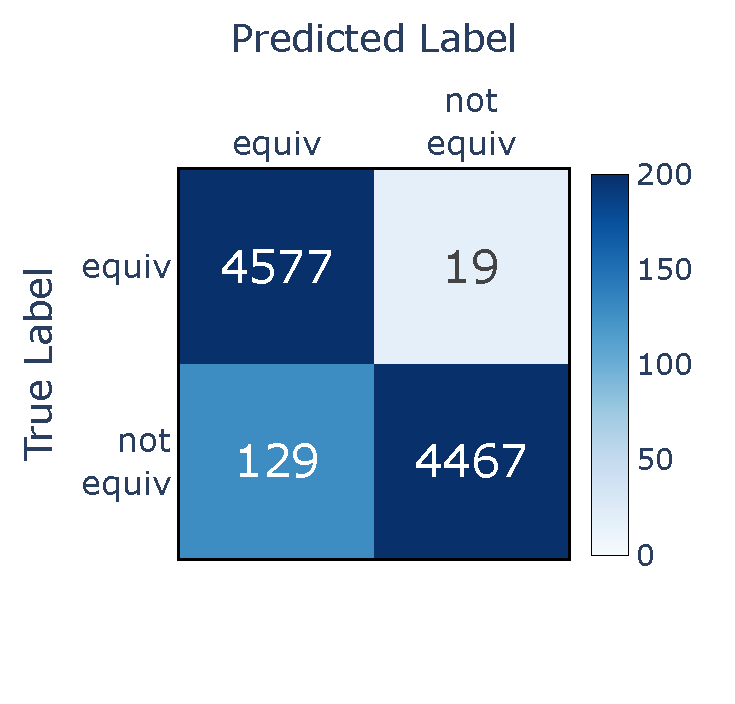
\includegraphics[width=0.194\textwidth,trim={29mm 23mm 26mm 0},clip]{cm_SFR_rf.pdf}
    }
    \captionsetup[subfigure]{oneside,margin={0cm,0cm}}
    \subfloat[SVM]{
        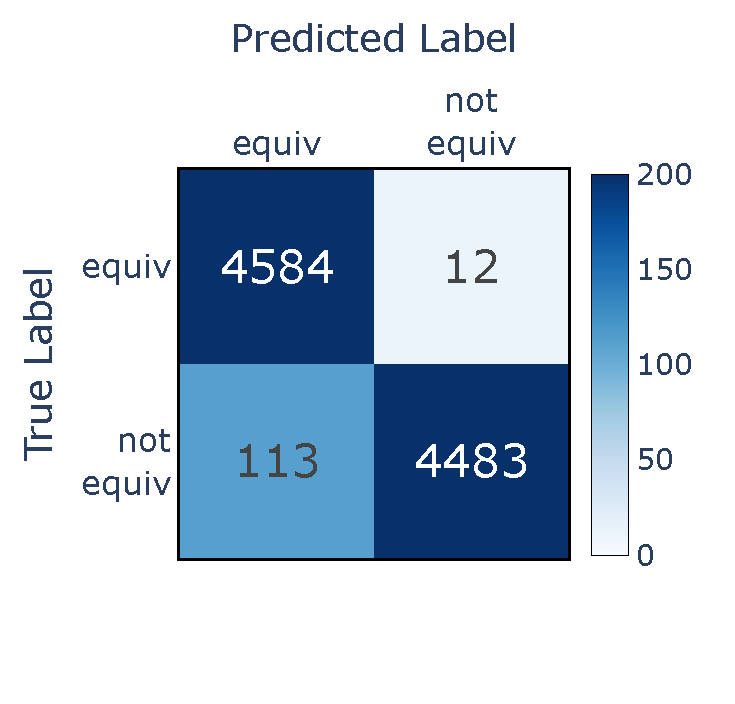
\includegraphics[width=0.194\textwidth,trim={29mm 23mm 26mm 0},clip]{cm_SFR_svm.pdf}
    }
    \captionsetup[subfigure]{oneside,margin={-1.25cm,0cm}}
    \subfloat[XGBoost]{
        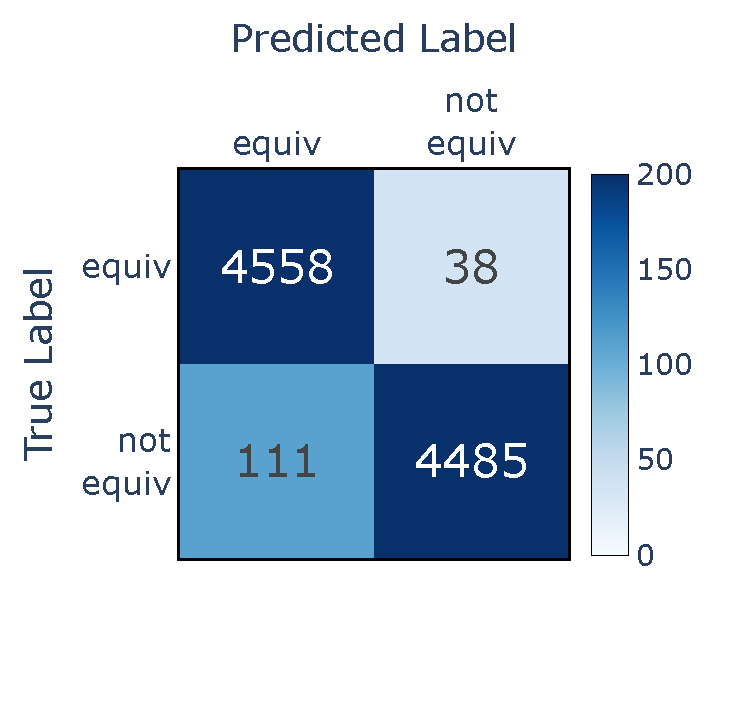
\includegraphics[width=0.246\textwidth,trim={29mm 23mm 7mm 0},clip]{cm_SFR_xgb.pdf}
    }
    \caption{SFR Confusion Matrices for Finalist Classifiers with Test Data}
\end{figure}


\chapter{Misclassification Analysis}
This appendix provides the full, unabridged text of representative misclassified course pairs discussed in Section~\ref{ch:4.6}, allowing for a direct, in-depth review of the error types.

\section{Most Misclassified Courses}\label{app:mostmiscls}
This is an inspection of the top 5 most misclassified courses across all classifiers and embedding models for both the training and test sets.

\begin{longtable}{ >{\baselineskip=12pt}c >{\baselineskip=12pt}p{0.9\textwidth} }
\captionsetup{skip=5pt}
\caption{Most Misclassified Courses (Training)}\label{tab:fp_overlap}\\
\toprule
\textbf{\textbf{Rank}} & \textbf{\textbf{Course}} \\
\midrule
\endhead
1 & CID: ENGL-120 \newline
Santa Barbara City College \newline
ENG-222 Survey of British Literature \newline
Offered only in the Spring semester. Survey of British literature during 1798-present, including fiction, poetry, drama and essays. Prerequisite: ENG 110 or ENG 110H\\
\midrule
2 & CID: JOUR-130 \newline
Fullerton College \newline
JOUR-271 F Introduction to Spansh-Language Reporting \newline
Advisory: Understanding of conversational Spanish. 54 hours lecture and 18 hours lab per term. This course will guide students in the methods and styles of reporting and writing in Spanish for print and online. It will prepare students to publish stories and photos on the campus' Spanish-language publication. The course also provides students with a general understanding of contemporary Spanish-speaking and Latino communities. (CSU) (Degree Credit)\\
\midrule
3 & CID: PHYS-140 \newline
Berkeley City College \newline
CHEM-30A Introductory General Chemistry \newline
Fundamental principles of general chemistry: Metric measurements, matter and energy, atomic structure, chemical nomenclature, chemical bonding, chemical reactions, stoichiometry, gas laws, nuclear chemistry; properties of liquids, solids, solutions, acids, and bases.\\
\midrule
4 & CID: SOCI-125 \newline
Compton College \newline
SOCI-120 Introduction to Statistics and Data Analysis for the Behavioral Sciences \newline
This course introduces students to lesbian, gay, bisexual, transgender, and queer studies. It is designed to analyze power, privilege, and oppression in connection to current macro and micro dynamics in society. Students will evaluate significant historical LGBTQ+ events that fostered changing society's views on sexual identities, as well as, events that have worked against advancing LGBTQ+ rights. In addition, students will evaluate various theories and concepts that attempt to explain the social construction of gender, sex, and sexuality. Furthermore, students can analyze socialization, cultural values, norms, intersectionality, and the unique challenges that impact LGBTQ+ communities.\\
\midrule
5 & CID: PHYS-200 \newline
Foothill College \newline
PHYS-4A General Physics (Calculus) \newline
Mathematics-physics interrelationships, classical Newtonian mechanics. Lecture and lab hours indicated are per week. This course includes 5 lecture hours and 3 lab hours per week.\\
\bottomrule
\end{longtable}

\begin{longtable}{ >{\baselineskip=12pt}c >{\baselineskip=12pt}p{0.9\textwidth} }
\captionsetup{skip=5pt}
\caption{Most Misclassified Courses (Test)}\label{tab:fp_overlap}\\
\toprule
\textbf{\textbf{Rank}} & \textbf{\textbf{Course}} \\
\midrule
\endhead
1 & CID: CDEV-100 \newline
Cerritos College \newline
CD-110 Child Development \newline
Examines the historical and current perspectives on diversity and inclusion and the impact of systemic societal influences on childrenÕs development, learning, and school experiences. Strategies for developmentally, culturally, and linguistically appropriate anti-bias curriculum will be explored as well as approaches to promote inclusive and anti-racist classroom communities. Includes self-reflection on the influence of teachersÕ own culture and life experiences on teaching and interactions with children and families.
Transfer Credit: CSU; UC\\
\midrule
2 & CID: ECE-230 \newline
Cerritos College \newline
CD-124 Teaching in a Diverse Society \newline
Introduces the appropriate use of assessment and observation tools and strategies to document young childrenÕ
s development and learning. The use of findings to inform and plan learning environments and experiences are
emphasized. Recording strategies, rating systems, portfolios, and multiple assessment tools will be
discussed, along with strategies for collaboration with families and professionals. 
Transfer Credit: CSU\\
\midrule
3 & CID: COMM-110 \newline
Saddleback College \newline
COMM-1 Communication Fundamentals \newline
Understand and use the processes of communication in making personal and social decisions in everyday life, including an understanding of problems and propositions; organization and development of ideas; evidence; methods of research, criticism and evaluation. Presentation of ideas in informative and persuasive contexts. Platform speaking experience will be required (formerly SP 1).\\
\midrule
4 & CID: CDEV-100 \newline
Cypress College \newline
PSY-145 C Child Psychology \newline
This course explores the physical, cognitive, communicative/linguistic, and socio-emotional development of the child from conception through adolescence across diverse cultures with an emphasis on the learning process. Education and teaching issues related to children are highlighted. (UC/CSU, AA GE, CSU GE, IGETC, CDEV 100)\\
\midrule
5 & CID: MUS-180 \newline
East Los Angeles College \newline
MUSIC-501 College Choir \newline
This course is an introduction to choral ensemble singing. Emphasis is on vocal technique and choral elements such as blend, intonation, diction, and music reading. Repertoire is chosen on the basis of group ability and represents historical and current styles of music. Students are required to perform in a public performance at the end of the semester.\\
\bottomrule
\end{longtable}

\section{False Positive: Topical Overlap}\label{app:topicoverlap}
This error occurs when courses cover the same broad subject but differ in critical dimensions such as academic level or their position in a curricular sequence. The model correctly identifies high semantic similarity but fails to capture the nuanced distinctions (e.g., Part I vs. Part II) that make the courses non-equivalent for articulation.

\begin{longtable}{ >{\baselineskip=12pt}p{0.45\textwidth} >{\baselineskip=12pt}p{0.45\textwidth} }
\captionsetup{skip=5pt}
\caption{FP Examples: Topical Overlap}\label{tab:fp_overlap}\\
\bottomrule\toprule
\textbf{\textbf{Course A}} & \textbf{\textbf{Course B}} \\
\bottomrule\toprule
\endhead
% Example 1: Sequential Physics
Evergreen Valley College \newline PHYS-004B (C-ID: PHYS-210) \newline General Physics & Foothill College \newline PHYS-4C (C-ID: PHYS-200) \newline General Physics (Calculus) \\
\midrule
This course is one of a three-semester series in calculus-based general physics, serving students majoring in engineering, chemistry, physics, mathematics and other sciences. It emphasizes conceptual aspects of electricity, magnetism, circuits, and Maxwell's equations, and requires quantitative analysis of real world situations. & Thermodynamics; mechanical, acoustical, and electromagnetic waves; optics. Lecture and lab hours indicated are per week. This course includes 5 lecture hours and 3 lab hours per week. \\
\bottomrule\toprule
% Example 2: Sequential English
East Los Angeles College \newline ENGLISH-205 (C-ID: ENGL-160) \newline English Literature I & East Los Angeles College \newline ENGLISH-206 (C-ID: ENGL-165) \newline English Literature II \\
\midrule
In this course, students read, discuss, and analyze major works of English literature from the Anglo-Saxon period to the late eighteenth century, to develop an understanding and appreciation of the poetry, fiction, and drama of these literary periods and to express that appreciation in a critical analysis. & This course surveys British Literature from the late 18th century emergence of the Romantics, such as Blake, Wordsworth, Coleridge, Byron, Shelley, and Keats; through the Victorian Era, writers such as Browning, Tennyson, Austen, Stevenson, Wilde, and Shaw; and into the early twentieth century, the rise of Modernism and after, writers such as Conrad, Eliot, Yeats, Woolf, Joyce, and Beckett. \\
\bottomrule\toprule
% Example 3: Intro vs. Bio-Psychology
Ventura College \newline PSY-V01 (C-ID: PSY-110) \newline Introduction to Psychology & Cabrillo College \newline PSYCH-4 (C-ID: PSY-150) \newline Introduction to Biological Psychology \\
\midrule
This course provides an overview of the scientific study of psychology in the areas of neuroscience, sensation and perception, states of consciousness, learning and memory, intellect and cognition, language, lifespan development and the influences of heredity and environment on behavior, motivation, sexuality, emotion, personality, stress and coping, psychological disorders, psychotherapy, and social relations. & Introduces the scientific study of the biological bases of behavior and its fundamental role in the neurosciences. Physiological, hormonal, and neurochemical mechanisms, and brain-behavior relationships underlying the psychological phenomena of sensation, perception, regulatory processes, emotion, learning, memory, and psychological disorders will be addressed. The course also notes historical scientific contributions and current research principles for studying brain-behavior relationships and mental processes. \\
\bottomrule\toprule
\end{longtable}

\section{False Positive: Ambiguous or Vague}\label{app:fpvague}
This error occurs when course descriptions are too brief or use generic, high-level language. This lack of specific detail increases ambiguity and can cause the model to identify semantic similarity between courses that are functionally distinct.

\begin{longtable}{ >{\baselineskip=12pt}p{0.45\textwidth}  >{\baselineskip=12pt}p{0.45\textwidth} }
\captionsetup{skip=5pt}
\caption{FP Examples: Ambiguous or Vague}\label{tab:fp_vague}\\
\bottomrule\toprule
\textbf{Course A} & \textbf{Course B} \\
\bottomrule\toprule
\endhead
% Example 1: Business Law
Cabrillo College \newline BUS-18 (C-ID: BUS-120) \newline Business Law & Long Beach City College \newline LAW-18 (C-ID: BUS-125) \newline Fundamental of Business Law \\
\midrule
Introduces the United States justice system, covering and relating criminal, civil, employment, torts and contract laws to business operations. History and nature of law, court systems, administrative agencies, crimes, cyber law, the formation and operation of contracts, corporate organization structures, ethical decisions and corporate responsibility and antitrust laws will be covered. & Formerly LAW 18A. This course is designed to explore the overall fundamental understanding of business law today. It examines the scope of how contracts and tort law affect the civil legal process as well as the nature of our current business environment. It is appropriate for students who wish to pursue a career in the business field. \\
\bottomrule\toprule
% Example 2: Communication
Cerritos College \newline COMM-132 (C-ID: COMM-140) \newline Fundamentals of Small Group Communication & Saddleback College \newline COMM-1 (C-ID: COMM-110) \newline Communication Fundamentals \\
\midrule
As an introduction to the fundamentals of group discussion, this course explores small group communication theories to examine group development; leadership in groups; group communication norms, and processes with emphasis on problem-solving, decision-making, and conflict-reduction techniques. Students will learn a variety of techniques to prepare and deliver group presentations. & Understand and use the processes of communication in making personal and social decisions in everyday life, including an understanding of problems and propositions; organization and development of ideas; evidence; methods of research, criticism and evaluation. Presentation of ideas in informative and persuasive contexts. Platform speaking experience will be required (formerly SP 1). \\
\bottomrule\toprule
\end{longtable}

\section{False Negative: Semantic Divergence}\label{app:semdiv}
This error occurs when two officially equivalent courses (i.e., sharing a C-ID) are described using vastly different terminology or pedagogical focus. The model correctly assesses the texts as semantically dissimilar; the failure lies in the inconsistency of the source data, where the ground truth asserts an equivalence that is not clearly supported by the text.

\begin{longtable}{ >{\baselineskip=12pt}p{0.45\textwidth}  >{\baselineskip=12pt}p{0.45\textwidth} }
\captionsetup{skip=5pt}
\caption{FN Examples: Semantic Divergence}\label{tab:fn_divergence}\\
\bottomrule\toprule
\textbf{\textbf{Course A}} & \textbf{Course B} \\
\bottomrule\toprule
\endhead
% Example 1: CDEV-100
Bakersfield College \newline CHDV-B21 (C-ID: CDEV-100) \newline Child Growth and Development: Birth Through Adolescence & Cerritos College \newline CD-110 (C-ID: CDEV-100) \newline Child Development \\
\midrule
This introductory course examines the major physical, psychosocial, and cognitive/language developmental milestones for children, both typical and atypical, from conception through adolescence. There will be an emphasis on interactions between maturational processes and environmental factors. While studying developmental theory and investigative research methodologies, students will observe children, evaluate individual differences and analyze characteristics of development at various stages. & Examines the historical and current perspectives on diversity and inclusion and the impact of systemic societal influences on children’s development, learning, and school experiences. Strategies for developmentally, culturally, and linguistically appropriate anti-bias curriculum will be explored as well as approaches to promote inclusive and anti-racist classroom communities. Includes self-reflection on the influence of teachers’ own culture and life experiences on teaching and interactions with children and families. \\
\bottomrule\toprule
% Example 2: ECE-230
Cerritos College \newline CD-124 (C-ID: ECE-230) \newline Teaching in a Diverse Society & Oxnard College \newline ECE-R107 (C-ID: ECE-230) \newline Teaching in a Diverse Society \\
\midrule
Introduces the appropriate use of assessment and observation tools and strategies to document young children’s development and learning. The use of findings to inform and plan learning environments and experiences are emphasized. Recording strategies, rating systems, portfolios, and multiple assessment tools will be discussed, along with strategies for collaboration with families and professionals. & This course examines the impact of various societal influences on the development of children's social identity. Students encounter that diversity is a major cultural trait of the United States, and recognize that schools reflect the societal makeup of our country. The course includes an identification of the main differences and similarities among various cultural groups and those of the mainstream culture. \\
\bottomrule\toprule
% Example 3: SOCI-160
Santa Barbara City College \newline SOC-106 (C-ID: SOCI-160) \newline Sociology of Deviance & Fullerton College \newline SOC-292 F (C-ID: SOCI-160) \newline Introduction to Criminology \\
\midrule
Examination of deviance and social control in contemporary society, using the sociological perspective. Focuses on the social processes involved in the construction of deviance, and its functions and impacts on individuals and society. Covers interpersonal and family violence; mental disorders; deviant sexuality; drug and alcohol use; and property, white-collar and organized crime. & This course is a study of theories of crimes and criminal behavior, including an explanation of crime, its causes, and how crime is measured. Major sociological and social science theories will be explored surrounding the issues of crime and criminal behavior. \\
\bottomrule\toprule
\end{longtable}

\section{False Negative: Incomplete or Vague}\label{app:fnvague}
This error arises when one or both course descriptions in an equivalent pair are too sparse or generic to provide sufficient textual signal for the model to establish a confident match. Unlike semantic divergence where both descriptions are detailed but different, here the issue is a lack of substantive, comparable information.

\begin{longtable}{ >{\baselineskip=12pt}p{0.45\textwidth}  >{\baselineskip=12pt}p{0.45\textwidth} }
\captionsetup{skip=5pt}
\caption{FN Examples: Incomplete or Vague}\label{tab:fn_incomplete}\\
\bottomrule\toprule
\textbf{Course A} & \textbf{Course B} \\
\bottomrule\toprule
\endhead
% Example 1: Field Geography
Cypress College \newline GEOG-202 C (C-ID: GEOG-160) \newline Field Geography - Physical & Palomar College \newline GEOG-195 (C-ID: GEOG-160) \newline Regional Field Studies in Geography \\
\midrule
Each separate offering of this course will occur in a unique location, studying unique circumstances and conditions in the field. Each course will employ its own combination of technical equipment, scientific instruments, and geotechniques. All courses will study the basic conceptual materials, with modifications associated with the location and the specific conditions encountered at each season. & Extended field studies of the geography of selected regions. Emphasis upon field observation and interpretation of climate, meteorology, vegetation, soils, and landforms. \\
\bottomrule\toprule
% Example 2: Physics
Imperial Valley College \newline PHYS-200 (C-ID: PHYS-205) \newline General Physics I & Moorpark College \newline PHYS-M20A (C-ID: PHYS-205) \newline Mechanics Solids and Fluids \\
\midrule
This course is designed to give an understanding of the fundamental principles of physics in the area of mechanics. & Introduces the basic principles of the mechanics of solids and fluids. Uses calculus to develop the subject matter. Covers kinematics, Newtonian mechanics including rotational dynamics, work, energy, fluid statics and dynamics, and simple harmonic motion. \\
\bottomrule\toprule
\end{longtable}

\section{False Negative: Labeling Errors}\label{app:labelerror}
This error arises when othere is a data entry error or the label is incorrect.

\begin{longtable}{ >{\baselineskip=12pt}p{0.45\textwidth}  >{\baselineskip=12pt}p{0.45\textwidth} }
\captionsetup{skip=5pt}
\caption{FN Examples: Data Entry or Labeling Error}\label{tab:fn_incomplete}\\
\bottomrule\toprule
\textbf{Course A} & \textbf{Course B} \\
\bottomrule\toprule
\endhead
% Example 1: Field Geography
Santa Barbara City College \newline PSY-150 (C-ID: SOCI-125) \newline Statistics for the Behavioral Sciences & Compton College \newline SOCI-120 (C-ID: SOCI-125) \newline Introduction to Statistics and Data Analysis for the Behavioral Sciences \\
\midrule
Principles and procedures of measurement, data analysis, probability, sampling theory and statistical significance. Covers basic descriptive statistics, including measures of linear relationships and standard scores. Covers the logic of hypothesis testing and inferential statistics up to analysis of variance, including a conceptual introduction to factorial designs. Students conduct analyses by hand and computer software. & This course introduces students to lesbian, gay, bisexual, transgender, and queer studies. It is designed to analyze power, privilege, and oppression in connection to current macro and micro dynamics in society. Students will evaluate significant historical LGBTQ+ events that fostered changing society's views on sexual identities, as well as, events that have worked against advancing LGBTQ+ rights. In addition, students will evaluate various theories and concepts that attempt to explain the social construction of gender, sex, and sexuality. Furthermore, students can analyze socialization, cultural values, norms, intersectionality, and the unique challenges that impact LGBTQ+ communities.\\
\bottomrule\toprule
\end{longtable}